%!TEX TS-program = pdflatexmk
\documentclass[cleanfoot]{asme2ej}

\usepackage[]{graphicx}
\graphicspath{ {images/} }

\usepackage{enumitem}
\usepackage{amsmath,amssymb}
\usepackage{textcomp}
\usepackage[urlcolor=blue,linkcolor=red,colorlinks=true]{hyperref}
\usepackage[autostyle, english=american]{csquotes}
\MakeOuterQuote{"}

\title{Exoplanet Open-Source Imaging Mission Simulator (EXOSIMS) \\ Interface Control Document}

%%% first author
\author{Christian Delacroix, Daniel Garrett, and Dmitry Savransky
    \affiliation{
    Sibley School of Mechanical and Aerospace Engineering\\
	Cornell University\\
	Ithaca, NY 14853
    }	
}

\def\mf{\mathbf}
\def\mb{\mathbb}
\def\mc{\mathcal}
\newcommand{\R}{\mathbf{r}}
\newcommand{\bc}{\mathbf{b}}
\newcommand{\mfbar}[1]{\mf{\bar{#1}}}
\newcommand{\mfhat}[1]{\mf{\hat{#1}}}
\newcommand{\bmu}{\boldsymbol{\mu}}
\newcommand{\blam}{\boldsymbol{\Lambda}}
\newcommand{\refeq}[1]{Equation  (\ref{#1})} 
\newcommand{\reftable}[1]{Table \ref{#1}} 
\newcommand{\refch}[1]{Chapter  \ref{#1}} 
\newcommand{\reffig}[1]{Figure \ref{#1}}
\newcommand{\refcode}[1]{Listing \ref{#1}}
\newcommand{\intd}[1]{\ensuremath{\,\mathrm{d}#1}}
\newcommand{\leftexp}[2]{{\vphantom{#2}}^{#1}\!{#2}}
\newcommand{\leftsub}[2]{{\vphantom{#2}}_{#1}\!{#2}}
\newcommand{\fddt}[1]{\ensuremath{\leftexp{\mathcal{#1}}{\frac{\mathrm{d}}{\mathrm{d}t}}}}
\newcommand{\fdddt}[1]{\ensuremath{\leftexp{\mathcal{#1}}{\frac{\mathrm{d}^2}{\mathrm{d}t^2}}}}
\newcommand{\omegarot}[2]{\ensuremath{\leftexp{\mathcal{#1}}{\boldsymbol{\omega}}^{\mathcal{#2}}}}


\begin{document}

\maketitle    

%%%%%%%%%%%%%%%%%%%%%%%%%%%%%%%%%%%%%%%%%%%%%%%%%%%%%%%%%%%%%%%%%%%%%%
\begin{abstract}
{\it This document describes the extensible, modular, open source software framework EXOSIMS.  EXOSIMS creates end-to-end simulations of space-based exoplanet imaging missions using stand-alone software modules.  The input/output interfaces of each module and interactions of modules with each other are presented to give guidance on mission specific modifications to the EXOSIMS framework. Last Update: \today}
\end{abstract}

\tableofcontents

%%%%%%%%%%%%%%%%%%%%%%%%%%%%%%%%%%%%%%%%%%%%%%%%%%%%%%%%%%%%%%%%%%%%%%
\begin{nomenclature}
\entry{EXOSIMS}{Exoplanet Open-Source Imaging Mission Simulator}
\entry{ICD}{Interface Control Document}
\entry{MJD}{Modified Julian Day}
\end{nomenclature}

%%%%%%%%%%%%%%%%%%%%%%%%%%%%%%%%%%%%%%%%%%%%%%%%%%%%%%%%%%%%%%%%%%%%%%
% INTRODUCTION
%%%%%%%%%%%%%%%%%%%%%%%%%%%%%%%%%%%%%%%%%%%%%%%%%%%%%%%%%%%%%%%%%%%%%%

\section{Introduction} 
Building confidence in a mission concept's ability to achieve its science goals is always desirable.  Unfortunately, accurately modeling the science yield of an exoplanet imager can be almost as complicated as designing the mission.  It is challenging to compare science simulation results and systematically test the effects of changing one aspect of the instrument or mission design.

EXOSIMS (Exoplanet Open-Source Imaging Mission Simulator) addresses this problem by generating ensembles of mission simulations for exoplanet direct imaging missions to estimate science yields. It is designed to allow systematic exploration of exoplanet imaging mission science yields.  It consists of stand-alone modules written in Python which may be modified without requiring modifications to other portions of the code. This allows EXOSIMS to be easily used to investigate new designs for instruments, observatories, or overall mission designs independently. This document describes the required input/output interfaces for the stand-alone modules to enable this flexibility.

\subsection{Purpose and Scope} % Rework this section
This Interface Control Document (ICD) provides an overview of the software framework of EXOSIMS and some details on its component parts.  As the software is intended to be highly reconfigurable, operational aspects of the code are emphasized over implementational details.  Specific examples are taken from the coronagraphic instrument under development for WFIRST.  The data inputs and outputs of each module are described. Following these guidelines will allow the code to be updated to accommodate new mission designs.

This ICD defines the input/output of each module and the interfaces between modules of the code.  This document is intended to guide mission planners and instrument designers in the development of specific modules for new mission designs.

%\subsection{Glossary}
%This section will contain definition of terms used throughout the document if needed.

\section{Overview}
The terminology used to describe the software implementation is loosely based upon object-oriented programing (OOP) terminology, as implemented by the Python language, in which EXOSIMS is built.  The term module can refer to the object class prototype representing the abstracted functionality of one piece of the software, an implementation of this object class which inherits the attributes and methods of the prototype, or an instance of this class.  Input/output definitions of modules refer to the class prototype.  Implemented modules refer to the inherited class definition.  Passing modules (or their outputs) means the instantiation of the inherited object class being used in a given simulation.  Relying on strict inheritance for all implemented module classes provides an automated error and consistency-checking mechanism.  The outputs of a given object instance may be compared to the outputs of the prototype.  It is trivial to pre-check whether a given module implementation will work within the larger framework, and this approach allows for flexibility and adaptability.

% \begin{figure}[ht]
%     \begin{center}
%         \begin{tabular}{c}
%              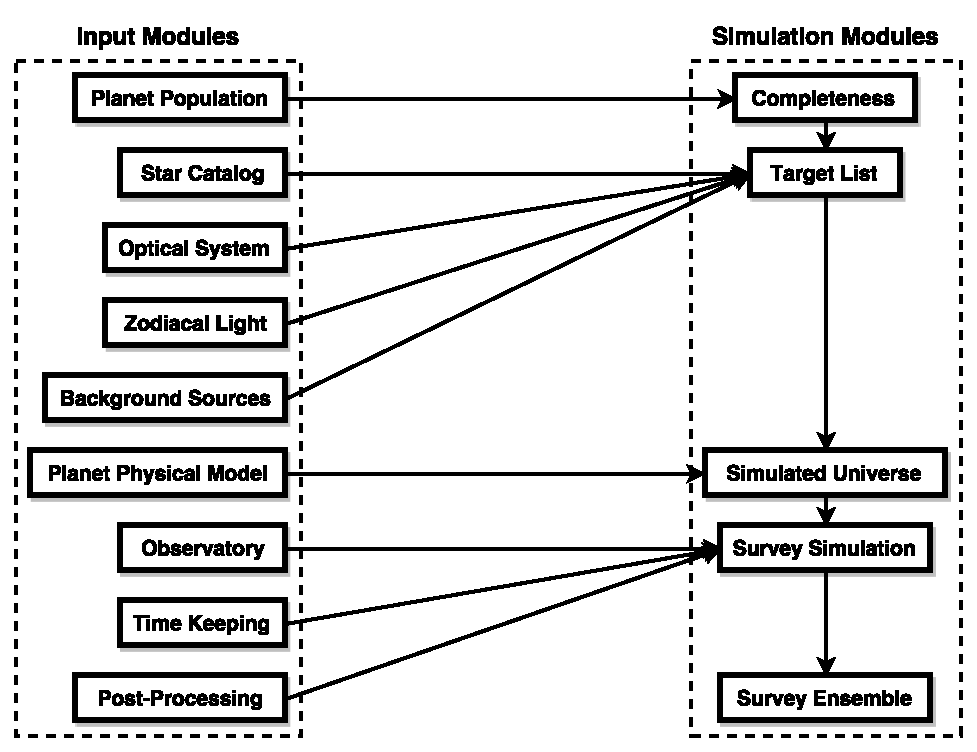
\includegraphics[width=0.9\textwidth]{codeflow5}
%         \end{tabular}
%     \end{center}
%     \caption{EXOSIMS modules. Each box represents a component software module that interacts with other modules as indicated by the arrows. The simulation modules pass all input modules along with their own output.  Thus, the Survey Ensemble module has access to all of the input modules and all of the upstream simulation modules.}
%     \label{figure_framework}
% \end{figure}

The overall framework of EXOSIMS is depicted in \reffig{fig:instantiation_tree} which shows all of the component software modules in the order in which they are instantiated in normal operation. The modules include the Optical System, Star Catalog, Planet Population, Observatory, Planet Physical Model, Time Keeping, Zodiacal Light, Background Sources, and Post-Processing modules and Target List, Simulated Universe, Survey Simulation, and Survey Ensemble modules.  Objects of all module classes can be instantiated independently, although most modules require the instantiation of other modules during their construction. Different implementations of the modules contain specific mission design parameters and physical descriptions of the universe, and will change according to mission and planet population of interest.  The upstream modules (including Target List, Simulated Universe, Survey Simulation, and Survey Ensemble modules) take information contained in the downstream modules and perform mission simulation tasks. The instantiation of an object of any of these modules requires the instantiation of one or more downstream module objects.  Any module may perform any number or kind of calculations using any or all of the input parameters provided.  The specific implementations are only constrained by their input and output specification contained in this document.
\begin{figure}[ht]
    \begin{center}
        \begin{tabular}{c}
             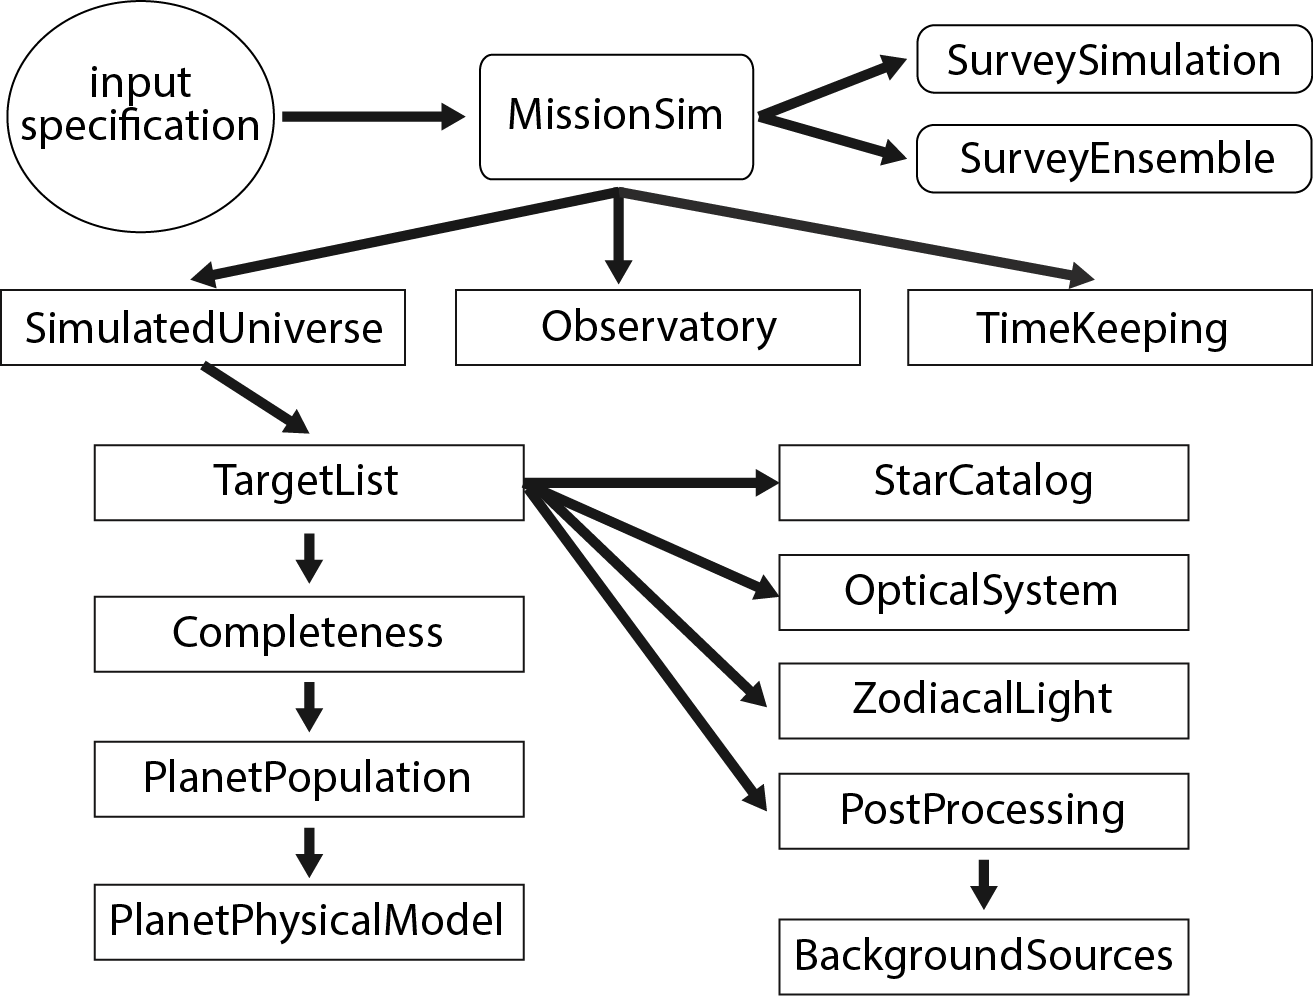
\includegraphics[width=0.7\textwidth]{instantiation_tree1}
        \end{tabular}
    \end{center}
    \caption{Schematic depiction of the instantiation path of all EXOSIMS modules.  The entry point to the backbone is the construction of a MissionSim object, which causes the instantiation of all other module objects.  All objects are instantiated in the order shown here, with SurveySimulation and SurveyEnsemble constructed last.  The arrows indicate calls to the object constructor, and object references to each module are always passed up directly to the top calling module, so that at the end of construction, the MissionSim object has direct access to all other modules as its attributes.}
    \label{fig:instantiation_tree}
\end{figure}

\begin{figure}[ht]
    \begin{center}
        \begin{tabular}{c}
             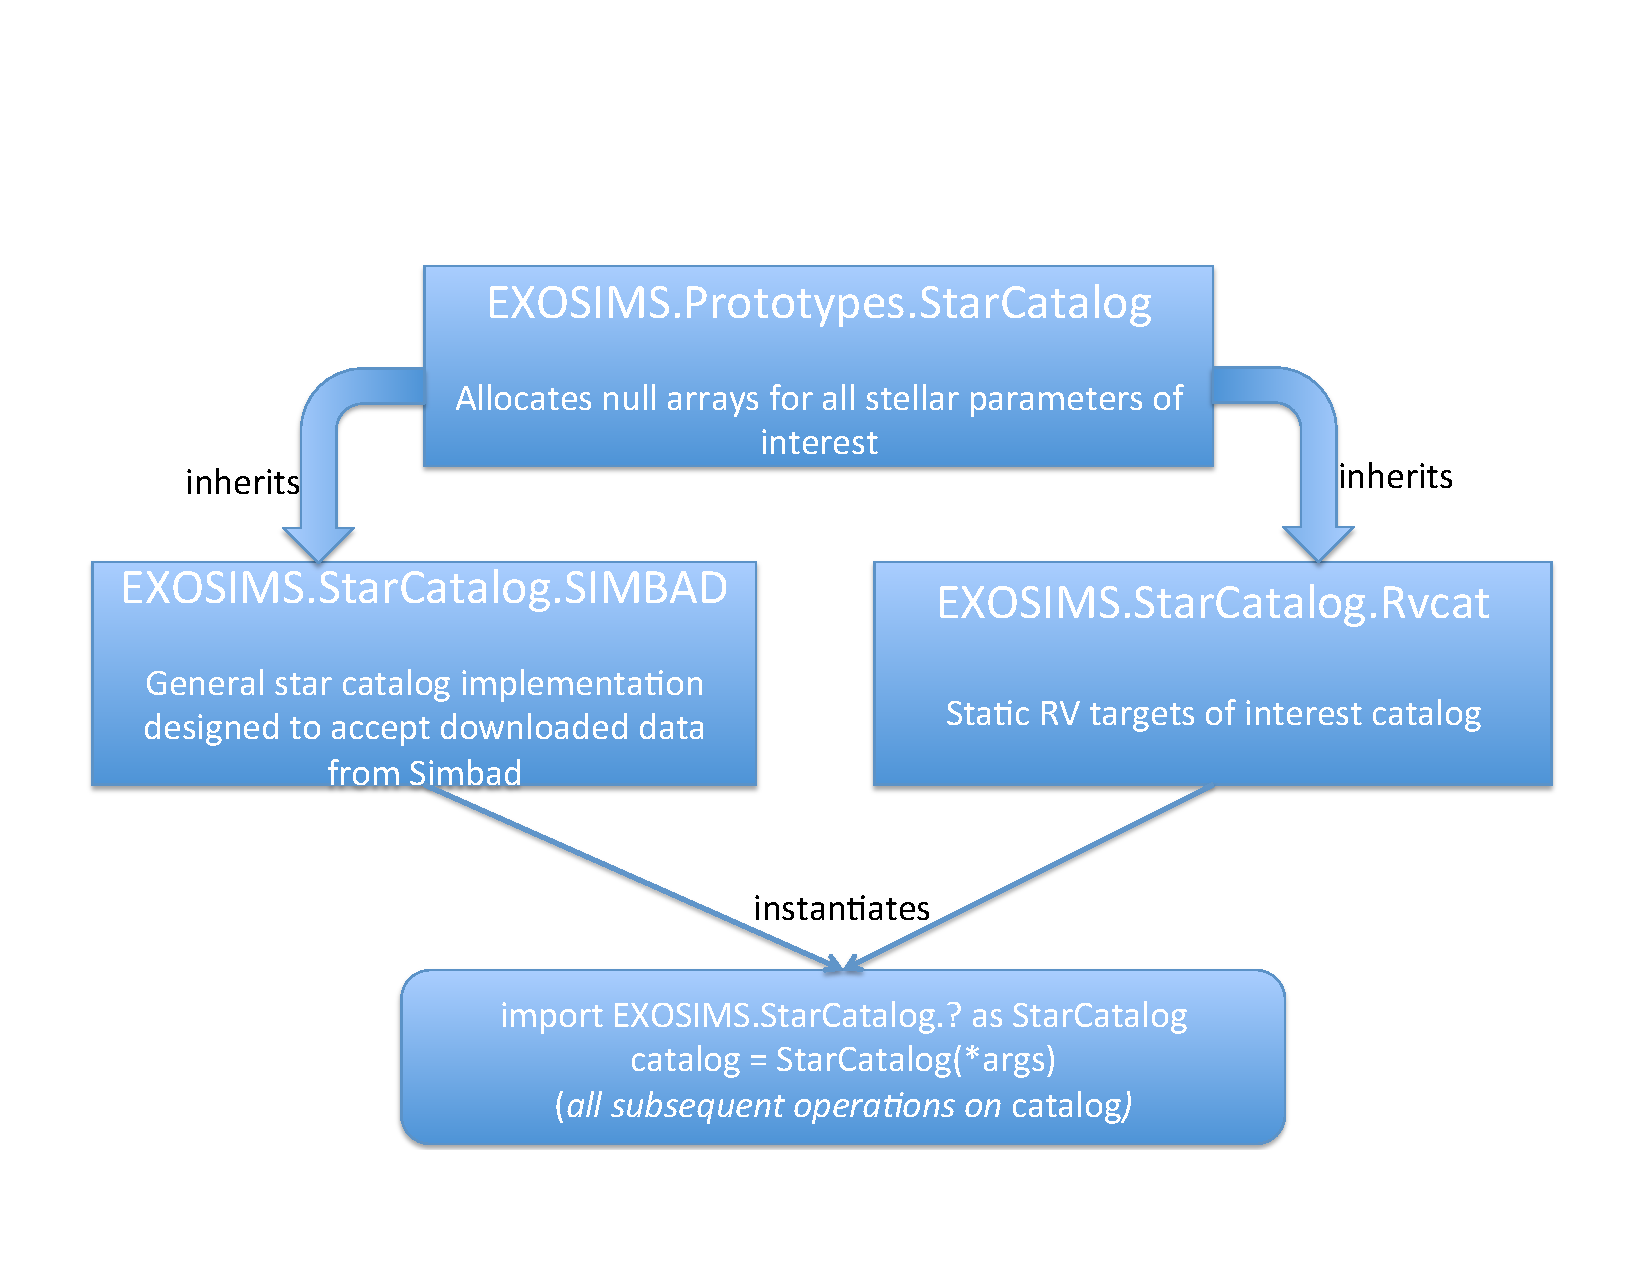
\includegraphics[width=0.75\textwidth]{starcatalog_flowdown}
        \end{tabular}
    \end{center}
    \caption{Schematic of a sample implementation for the three module layers for the Star Catalog module. The Star Catalog prototype (top row) is immutable, specifies the input/output structure of the module along with all common functionality, and is inherited by all Star Catalog class implementations (middle row).  In this case, two different catalog classes are shown: one that reads in data from a SIMBAD catalog dump, and one which contains only information about a subset of known radial velocity targets.  The object used in the simulation (bottom row) is an instance of one of these classes, and can be used in exactly the same way in the rest of the code due to the common input/output scheme.}
    \label{fig:starcatalog_flowdown}
\end{figure}

\begin{figure}[ht]
    \begin{center}
        \begin{tabular}{c}
             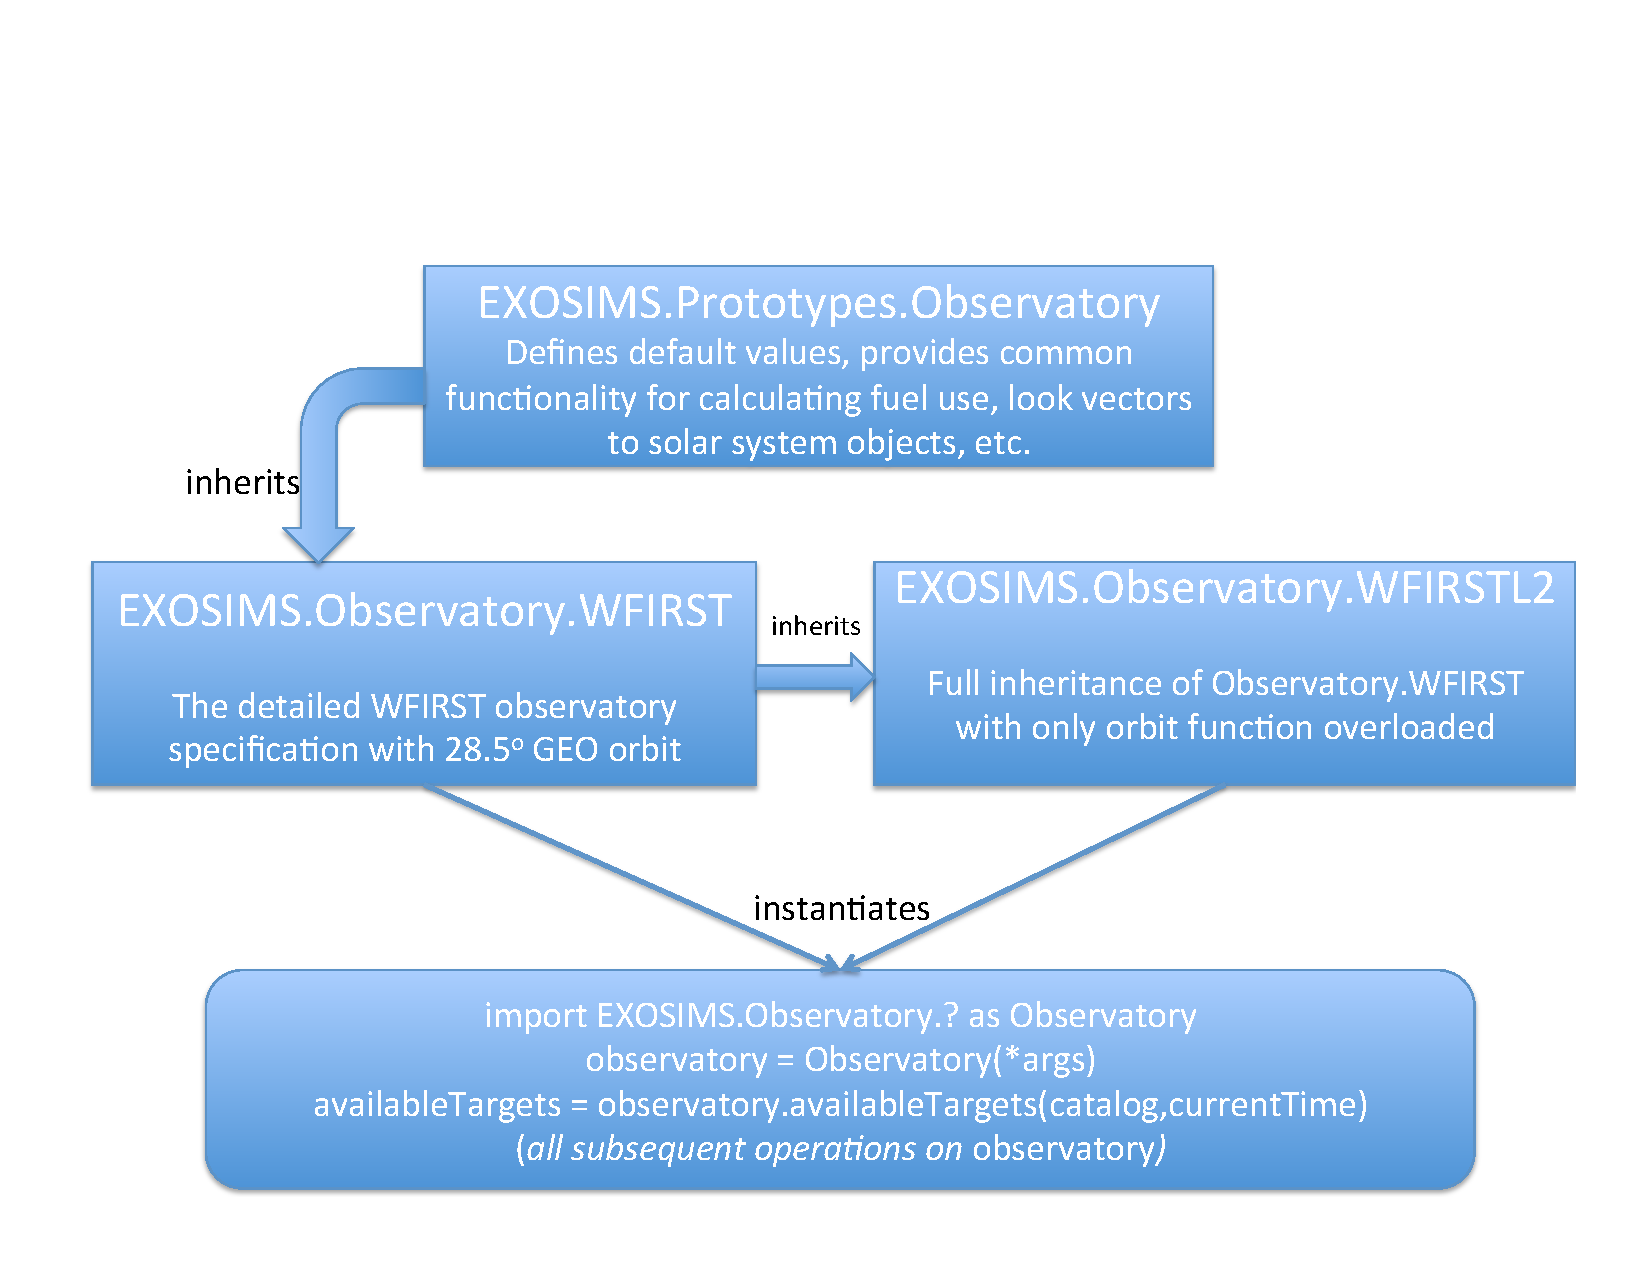
\includegraphics[width=0.75\textwidth]{observatory_flowdown}
        \end{tabular}
    \end{center}
    \caption{Schematic of a sample implementation for the three module layers for the Observatory module. The Observatory prototype (top row) is immutable, specifies the input/output structure of the module along with all common functionality, and is inherited by all Observatory class implementations (middle row).  In this case, two different observatory classes are shown that differ only in the definition of the observatory orbit.  Therefore, the second implementation inherits the first (rather than directly inheriting the prototype) and overloads only the orbit method. The object used in the simulation (bottom row) is an instance of one of these classes, and can be used in exactly the same way in the rest of the code due to the common input/output scheme.}
    \label{fig:observatory_flowdown}
\end{figure}

Figures \ref{fig:starcatalog_flowdown} and \ref{fig:observatory_flowdown} show schematic representations of the three different aspects of a module, using the Star Catalog and Observatory modules as examples, respectively.  Every module has a specific prototype that sets the input/output structure of the module and encodes any common functionality for all module class implementations.  The various implementations inherit the prototype and add/overload any attributes and methods required for their particular tasks, limited only by the preset input/output scheme.  Finally, in the course of running a simulation, an object is generated for each module class selected for that simulation.  The generated objects can be used in exactly the same way in the downstream code, regardless of what implementation they are instances of, due to the strict interface defined in the class prototypes.

For lower level (downstream) modules, the input specification is much more loosely defined than the output specification, as different implementations may draw data from a wide variety of sources.  For example, the star catalog may be implemented as reading values from a static file on disk, or may represent an active connection to a local or remote database.  The output specification for these modules, however, as well as both the input and output for the upstream modules, is entirely fixed so as to allow for generic use of all module objects in the simulation.


\section{Global Specifications}
Common references (units, frames of reference, etc.) are required to ensure interoperability between the modules of EXOSIM.  All of the references listed below must be followed.

\begin{description}
    \item[Common Epoch] \hfill \\ J2000
    \item[Common Reference Frame] \hfill \\ Heliocentric Equatorial (HE)
\end{description}

\subsection{Python Packages} 
EXOSIMS is an open source platform.  As such, packages and modules may be imported and used for calculations within any of the stand-alone modules.  The following commonly used Python packages are used for the WFIRST-specific implementation of EXOSIMS:

\texttt{
\begin{itemize}
    \item astropy
        \begin{itemize}
            \item astropy.constants
            \item astropy.coordinates
            \item astropy.time
            \item astropy.units
        \end{itemize}
    \item copy
    \item hashlib
    \item importlib
    \item numpy
        \begin{itemize}
            \item numpy.linalg 
        \end{itemize}
    \item os
        \begin{itemize}
            \item os.path 
        \end{itemize}
    \item pickle/cPickle
    \item scipy
        \begin{itemize}
            \item scipy.io
            \item scipy.special
            \item scipy.interpolate
        \end{itemize}
    \item h5py (\emph{optional})
    \item jplephem (\emph{optional})
\end{itemize}
}

Additionally, while not required for running the survey simulation, \verb+matplotlib+ is used for visualization of the results.

\subsection{Coding Conventions}
In order to allow for flexibility in using alternate or user-generated module implementations, the only requirement on any module is that it inherits (either directly or by inheriting another module implementation that inherits the prototype) the appropriate prototype.  It is similarly expected (although not required) that the prototype constructor will be called from the constructor of the newly implemented class.  An example of an Optical System module implementation follows:

\begin{verbatim}
from EXOSIMS.Prototypes.OpticalSystem import OpticalSystem

class ExampleOpticalSystem(OpticalSystem):
    
    def __init__(self, **specs):
                
        OpticalSystem.__init__(self, **specs)
        
        ...

\end{verbatim}

\emph{Note that the filename must match the class name for all modules.}

\subsubsection{Module Type}
It is always possible to check whether a module is an instance of a given prototype, for example:
\begin{verbatim}
isinstance(obj,EXOSIMS.Prototypes.Observatory.Observatory)
\end{verbatim}
However, it can be tedious to look up all of a given object's base classes so, for convenience, every prototype will provide a private variable \verb+_modtype+, which will always return the name of the prototype and should not be overwritten by any module code.  Thus, if the above example evaluates as \verb+True+, \verb+obj._modtype+ will return \verb+Observatory+.

\subsubsection{Callable Attributes}
Certain module attributes must be represented in a way that allows them to be parametrized by other values.  For example, the instrument throughput and contrast are functions of both the wavelength and the angular separation, and so must be encodable as such in the optical system module.  To accommodate this, as well as simpler descriptions where these parameters may be treated as static values, these and other attributes are defined as `callable'.  This means that they must be set as objects that can be called in the normal Python fashion, i.e., \verb+object(arg1,arg2,...)+.  

These objects can be function definitions defined in the code, or imported from other modules.  They can be \href{https://docs.python.org/2/reference/expressions.html#lambda}{lambda expressions} defined inline in the code.  Or they can be callable object instances, such as the various \href{http://docs.scipy.org/doc/scipy/reference/interpolate.html}{scipy interpolants}.  In cases where the description is just a single value, these attributes can be defined as dummy functions that always return the same value, for example:
\begin{verbatim}
def throughput(wavelength,angle):
     return 0.5
\end{verbatim}
or even more simply:
\begin{verbatim}
throughput = lambda wavelength,angle: 0.5
\end{verbatim}
%%%%%%%%%%%%%%%%%%%%%%%%%%%%%%%%%%%%%%%%%%%%%%%%%%%%%%%%%%%%%%%%%%%%
% BACKBONE
%%%%%%%%%%%%%%%%%%%%%%%%%%%%%%%%%%%%%%%%%%%%%%%%%%%%%%%%%%%%%%%%%%%%

\section{Backbone}
By default, the simulation execution will be performed via the backbone.  This will consist of a limited set of functions that will primarily be tasked with parsing the input specification described below, and then creating the specified instances of each of the framework modules, detailed in \S\ref{sec:modules}.  The backbone functionality will primarily be implemented in the \mbox{MissionSim} class, whose constructor will take the input script file (\S\ref{sec:inputspec}) and generate instances of all module objects, including the SurveySimulation (\S\ref{sec:surveysim}) and SurveyEnsemble modules, which will contain the functions to run the survey simulations. Any mission-specific execution variations will be introduced by method overloading in the inherited survey simulation implementation. \reffig{fig:instantiation_tree} provides a graphical description of the instantiation order of all module objects.


A simulation specification is a single JSON-formatted (\url{http://json.org/}) file that encodes user-settable parameters and module names.  The backbone will contain a reference specification with \emph{all} parameters and modules set via defaults in the constructors of each of the modules.  In the initial parsing of the user-supplied specification, it will be merged with the reference specification such that any fields not set by the user will be assigned to their reference (default) values.   Each instantiated module object will contain a dictionary called \verb+_outspec+, which, taken together, will form the full specification for the current run (as defined by the loaded modules).  This specification will be written out to a json file associated with the output of every run.  \emph{Any specification added by a user implementation of any module must also be added to the \_outspec dictionary}.  The assembly of the full output specification is provided by MissionSim method \verb+genOutSpec+.

The backbone will also contain a specification parser that will check specification files for internal consistency.  For example, if modules carry mutual dependencies, the specification parser will return an error if these are not met for a given specification.  Similarly, if modules are selected with optional top level inputs, warnings will be generated if these are not set in the same specification files.

In addition to the specification parser, the backbone will contain a method for comparing two specification files and returning the difference between them.  Assuming that the files specify all user-settable values, this will be equivalent to simply performing a \verb+diff+ operation on any POSIX system.  The backbone diff function will add in the capability to automatically fill in unset values with their defaults.  For every simulation (or ensemble), an output specification will be written to disk along with the simulation results with all defaults used filled in.

%The backbone will also contain an interactive function to help users generate specification files via a series of questions. 

\subsection{Specification Format}\label{sec:inputspec}
The JSON specification file will contain a series of objects with members enumerating various user-settable parameters, top-level members for universal settings (such as the mission lifetime) and arrays of objects for multiple related specifications, such as starlight suppression systems and science instruments.  The specification file must contain a \verb+modules+ dictionary listing the module names (or paths on disk to user-implemented classes) for all modules.

\begin{verbatim}
{
    "FAP": 3e-07,
    "FAdMag0": 15,
    "IWA": 0.15,
    "Irange": [
        0.0,
        180.0
    ],
    "MDP": 0.001,
    "Mprange": [
        1.0,
        4131.0
    ],
    "OBduration": 0,
    "OWA": 0.557002,
    "Orange": [
        0.0,
        360.0
    ],
    "Rprange": [
        1.0,
        22.6
    ],
    "WA0": 0.289498,
    "WAint": 0.3,
    "arange": [
        0.1,
        100.0
    ],
    "charMargin": 0.15,
    "checkKeepoutEnd": true,
    "coMass": 5800.0,
    "constrainOrbits": false,
    "currentTimeAbs": 60634.0,
    "currentTimeNorm": 0.0,
    "dMag0": 22.5,
    "dMagLim": 22.5,
    "dMagint": 22.5,
    "erange": [
        0.01,
        0.99
    ],
    "esigma": 0.25,
    "extendedLife": 0.0,
    "forceStaticEphem": false,
    "havejplephem": true,
    "intCutoff": 15.0,
    "keepStarCatalog": false,
    "koAngleMax": 90.0,
    "koAngleMin": 45.0,
    "koAngleMinEarth": 45.0,
    "koAngleMinMoon": 45.0,
    "koAngleSmall": 1.0,
    "magEZ": 22.0,
    "magZ": 23.0,
    "minComp": 0.0,
    "missionLife": 5.0,
    "missionPortion": 0.0493150685,
    "missionStart": 60634.0,
    "modules": {
        "BackgroundSources": "BackgroundSources",
        "Completeness": "GarrettCompleteness",
        "Observatory": "WFIRSTObservatoryL2",
        "OpticalSystem": "Nemati",
        "PlanetPhysicalModel": "Forecaster",
        "PlanetPopulation": "KeplerLike2",
        "PostProcessing": "PostProcessing",
        "SimulatedUniverse": "KeplerLikeUniverse",
        "StarCatalog": "EXOCAT1",
        "SurveyEnsemble": "SurveyEnsemble",
        "SurveySimulation": "SurveySimulation",
        "TargetList": "TargetList",
        "TimeKeeping": "TimeKeeping",
        "ZodiacalLight": "Stark"
    },
    "nVisitsMax": 5,
    "ntFlux": 1,
    "obscurFac": 0.1724,
    "observingModes": [
        {
            "SNR": 5,
            "detectionMode": true,
            "instName": "imager",
            "radDos": 0.5,
            "systName": "HLC-565"
        },
        {
            "SNR": 10,
            "instName": "spectro",
            "lam": 660,
            "radDos": 1.0,
            "systName": "SPC-660"
        }
    ],
    "occulterSep": 55000.0,
    "ppFact": 0.1,
    "prange": [
        0.083,
        0.882
    ],
    "pupilDiam": 2.37,
    "ref_Time": 0.2,
    "ref_dMag": 3.0,
    "scaleOrbits": false,
    "scienceInstruments": [
        {
            "CIC": 0.01,
            "ENF": 1.0,
            "FoV": 9.5,
            "PCeff": 0.8,
            "QE": "$HOME/Data/QEfile.fits",
            "Rs": 1.0,
            "fnumber": 60.97706197560175,
            "focal": 144.51563688217615,
            "idark": 0.000114,
            "lenslSamp": 1.0,
            "name": "imager",
            "optics": 0.518018590965876,
            "pixelNumber": 1024,
            "pixelScale": 0.0185546875,
            "pixelSize": 1.3e-05,
            "sread": 0.0,
            "texp": 100.0
        },
        {
            "CIC": 0.01,
            "ENF": 1.0,
            "FoV": 1.0,
            "PCeff": 0.8,
            "QE": "$HOME/Data/QEfile.fits",
            "Rs": 50.0,
            "fnumber": 575.4526999602537,
            "focal": 1363.8228989058011,
            "idark": 0.000114,
            "lenslSamp": 2.0,
            "name": "spectro",
            "optics": 0.465846901959329,
            "pixelNumber": 76,
            "pixelScale": 0.02631578947368421,
            "pixelSize": 0.000174,
            "sread": 0.0,
            "texp": 100.0
        }
    ],
    "settlingTime": 0.5,
    "shapeFac": 0.7853981633974483,
    "smaknee": 30.0,
    "starlightSuppressionSystems": [
        {
            "BW": 0.1,
            "IWA": 0.15,
            "OWA": 0.428996,
            "core_area": "$HOME/Data/area.fits",
            "core_contrast": 1e-10,
            "core_mean_intensity": "$HOME/Data/mean_intensity.fits",
            "core_platescale": 0.3,
            "core_thruput": "$HOME/Data/thruput.fits",
            "deltaLam": 56.5,
            "lam": 565.0,
            "name": "HLC-565",
            "occ_trans": "$HOME/Data/occ_trans.fits",
            "occulter": false,
            "ohTime": 0.5,
            "optics": 0.983647,
            "samp": 10.0
        },
        {
            "BW": 0.18,
            "IWA": 0.208876,
            "OWA": 0.557002,
            "core_area": "$HOME/Data/area.fits",
            "core_contrast": 1e-10,
            "core_mean_intensity": "$HOME/Data/mean_intensity.fits",
            "core_platescale": 0.3,
            "core_thruput": "$HOME/Data/thruput.fits",
            "deltaLam": 118.8,
            "lam": 660.0,
            "name": "SPC-660",
            "occ_trans": "$HOME/Data/occ_trans.fits",
            "occulter": false,
            "ohTime": 0.5,
            "optics": 0.9154706,
            "samp": 10.0
        }
    ],
    "staticStars": true,
    "waitMultiple": 2.0,
    "waitTime": 1.0,
    "wrange": [
        0.0,
        360.0
    ]
}
\end{verbatim}

\subsection{Modules Specification}
The final array in the input specification  (\verb+modules+) is a list of all the modules that define a particular simulation.  This is the only part of the specification that will not be filled in by default if a value is missing - each module must be explicitly specified. The order of the modules in the list is arbitrary, so long as they are all present. 

If the module implementations are in the appropriate subfolder in the EXOSIMS tree, then they can be specified by the module name.  However, if you wish to use an implemented module outside of the EXOSIMS directory, then you need to specify it via its full path in the input specification.

\emph{All modules, regardless of where they are stored on disk must inherit the appropriate prototype.}

\subsection{Universal Parameters}
These parameters apply to all simulations, and are described in detail in their specific module definitions:

\begin{itemize}[leftmargin=1.5in,font={\ttfamily}]

\item[\textbf{MissionSim}]
\item[verbose] (boolean) Boolean used to create the vprint function, equivalent to the python print function with an extra verbose toggle parameter (True by default). The vprint function can be accessed by all modules from EXOSIMS.util.vprint.
\item[seed] (integer) Number used to seed the NumPy generator. Generated randomly by default.
\item[logfile] (string) Path to the log file. If None, logging is turned off. If supplied but empty string (''), a temporary file is generated.
\item[loglevel] (string) The level of log, defaults to 'INFO'. Valid levels are: CRITICAL, ERROR, WARNING, INFO, DEBUG (case sensitive).

\item[\textbf{PlanetPopulation}]
\item[arange] (float) 1$\times$2 list of semi-major axis range in units of $ AU $. 
\item[erange] (float) 1$\times$2 list of eccentricity range.
\item[Irange] (float) 1$\times$2 list of inclination range in units of $ deg $.  
\item[Orange] (float) 1$\times$2 list of ascension of the ascending node range in units of $ deg $.  
\item[wrange] (float) 1$\times$2 list of argument of perigee range in units of $ deg $. 
\item[prange] (float) 1$\times$2 list of planetary geometric albedo range.  
\item[Rprange] (float) 1$\times$2 list of planetary radius range in Earth radii.  
\item[Mprange] (float) 1$\times$2 list of planetary mass range in Earth masses.  
\item [scaleOrbits] (boolean) True means planetary orbits are scaled by the square root of stellar luminosity. 
\item[constrainOrbits] (boolean) True means planetary orbits are constrained to never leave the semi-major axis range (arange).
\item[eta] (float) The average occurrence rate of planets per star for the entire population.

\item[\textbf{OpticalSystem}]
\item[obscurFac] (float) Obscuration factor due to secondary mirror and spiders.
\item[shapeFac] (float)  Telescope aperture shape factor.
\item[pupilDiam] (float) Entrance pupil diameter in units of $m$.
\item[IWA] (float) Fundamental Inner Working Angle in units of $ arcsec $. No planets can ever be observed at smaller separations.
\item[OWA] (float) Fundamental Outer Working Angle in units of $ arcsec $. Set to $ Inf $ for no OWA. JSON values of 0 will be interpreted as $ Inf $.
\item[intCutoff] (float)  Maximum allowed integration time in units of $ day $.
\item[dMag0] (float) Favorable planet delta magnitude value used to calculate the minimum integration times for inclusion in target list.
\item[WA0] (float) Instrument working angle value used to calculate the minimum integration times for inclusion in target list, in units of $arcsec$.
\item[scienceInstruments] (list of dicts) Contains specific attributes of all science instruments. 
\item[starlight-]
\item[SuppressionSystems] (list of dicts) Contains specific attributes of all starlight suppression systems.
\item[observingModes] (list of dicts) Contains specific attributes of all observing modes. 

\item[\textbf{ZodiacalLight}]
\item[magZ] (float) 1 zodi brightness magnitude (per arcsec2).
\item[magEZ] (float) 1 exo-zodi brightness magnitude (per arcsec2).
\item[varEZ] (float) exo-zodiacal light variation (variance of log-normal distribution).

\item[\textbf{PostProcessing}]
\item[FAP] (float) False Alarm Probability.
\item[MDP] (float) Missed Detection Probability.
\item[ppFact] (float, callable) Post-processing contrast factor, between 0 and 1.
\item[FAdMag0] (float, callable) Minimum delta magnitude that can be obtained by a false alarm.

\item[\textbf{Completeness}]
\item[dMagLim] (float) Limiting planet-to-star delta magnitude for completeness.
\item[minComp] (float) Minimum completeness value for inclusion in target list.

\item[\textbf{TargetList}]
\item[staticStars] (boolean) Boolean used to force static target positions set at mission start time.
\item[keepStarCatalog] (boolean) Boolean representing whether to delete the star catalog after assembling the target list.  If true, object reference will be available from TargetList object.

\item[\textbf{Observatory}]
\item[koAngleMin] (float) Telescope minimum keepout angle in units of $deg$. 
\item[koAngleMinMoon] (float) Telescope minimum keepout angle in units of $deg$, for the Moon only.
\item[koAngleMinEarth] (float) Telescope minimum keepout angle in units of $deg$, for the Earth only.
\item[koAngleMax] (float) Telescope maximum keepout angle (for occulter) in units of $deg$. 
\item[koAngleSmall] (float) Telescope keepout angle for smaller (angular size) bodies in units of $deg$. 
\item[checkKeepoutEnd] (boolean) Boolean signifying if the keepout method must be called at the end of each observation.
\item[settlingTime] (float) Amount of time needed for observatory to settle after a repointing in units of $ day $.
\item[thrust] (float) Occulter slew thrust in units of $ mN $.
\item[slewIsp] (float) Occulter slew specific impulse in units of $ s $.
\item[scMass] (float) Occulter (maneuvering spacecraft) initial wet mass in units of $ kg $. 
\item[dryMass] (float) Occulter (maneuvering spacecraft) dry mass in units of $ kg $. 
\item[coMass] (float) Telescope (or non-maneuvering spacecraft) mass in units of $ kg $. 
\item[occulterSep] (float) Occulter-telescope distance in units of $ km $. 
\item[skIsp] (float) Specific impulse for station keeping in units of $ s $. 
\item[defburnPortion] (float) Default burn portion for slewing.
\item[checkKeepoutEnd] (boolean) Boolean signifying if the keepout method must be called at the end of each observation.
\item[forceStaticEphem]  (boolean) Force use of static solar system ephemeris if set to True, even if jplephem module is present.
\item[spkpath] (string) Full path to SPK kernel file.

\item[\textbf{TimeKeeping}]
\item[missionLife] (float) The total mission lifetime in units of $ year $.  When the mission time is equal or greater to this value, the mission simulation stops.
\item[missionPortion] (float) The portion of the mission dedicated to exoplanet science, given as a value between 0 and 1. The mission simulation stops when the total integration time plus observation overhead time is equal to the missionLife $\times$ missionPortion.
\item[extendedLife] (float) Extended mission time in units of $ year $.  Extended life typically differs from the primary mission in some way---most typically only revisits are allowed
\item[missionStart] (float) Mission start time in $ MJD $. 
\item[OBduration] (float) Default allocated duration of observing blocks, in units of $day$. If no OBduration was specified, a new observing block is created for each new observation in the SurveySimulation module.
\item[waitTime] (float) Default allocated duration to wait in units of $day$, when the Survey Simulation does not find any observable target.
\item[waitMultiple] (float) Multiplier applied to the wait time in case of repeated empty lists of observable targets, which makes the wait time grow exponentially. 

\item[\textbf{SurveySimulation}]
\item[nt\_flux] (integer) Observation time sampling, to determine the integration time interval.
\item[nVisitsMax] (integer) Maximum number of observations (in detection mode) per star. 
\item[charMargin] (float) Integration time margin for characterization. 
\item[seed] (integer) Random seed used to make all random number generation reproducible.
\item[WAint] (float) Working angle used for integration time calculation in units of $arcsec$.
\item[dMagint] (float) Delta magnitude used for integration time calculation.


\end{itemize}

\section{Module Specifications}\label{sec:modules}
The lower level modules include Planet Population, Star Catalog, Optical System, Zodiacal Light, Background Sources, Planet Physical Model, Observatory, Time Keeping, and Post-Processing.  These modules encode and/or generate all of the information necessary to perform mission simulations.  The specific mission design determines the functionality of each module, while inputs and outputs of these modules remain the same (in terms of data type and variable representations).  

The upstream modules include Completeness, Target List, Simulated Universe, Survey Simulation and Survey Ensemble. These modules perform methods which require inputs from one or more downstream modules as well as calling function implementations in other upstream modules. 

This section defines the functionality, major tasks, input, output, and interface of each of these modules. Every module constructor must always accept a keyword dictionary (\verb+**spec+) representing the contents of the specification JSON file organized into a Python dictionary. The descriptions below list out specific keywords that are pulled out by the prototype constructors of each of the modules, but implemented constructors may include additional keywords (so long as they correctly call the prototype constructor).  In all cases, if a given \verb+key:value+ pair is missing from the dictionary, the appropriate object attributes will be assigned the default values listed.


% STAR CATALOG

\subsection{Star Catalog} \label{sec:starcatalog}
The Star Catalog module includes detailed information about potential target stars drawn from general databases such as SIMBAD, mission catalogs such as Hipparcos, or from existing curated lists specifically designed for exoplanet imaging missions.  Information to be stored, or accessed by this module will include target positions and proper motions at the reference epoch, catalog identifiers (for later cross-referencing), bolometric luminosities, stellar masses, and magnitudes in standard observing bands.  Where direct measurements of any value are not available, values are synthesized from ancillary data and empirical relationships, such as color relationships and mass-luminosity relations.

This module does not provide any functionality for picking the specific targets to be observed in any one simulation, nor even for culling targets from the input lists where no observations of a planet could take place.  This is done in the Target List module as it requires interactions with the Planet Population (to determine the population of interest), Optical System (to define the capabilities of the instrument), and Observatory (to determine if the view of the target is unobstructed) modules.

\subsubsection{Star Catalog Object Attribute Initialization} 
The Star Catalog prototype creates empty 1D NumPy ndarrays for each of the output quantities listed below.  Specific Star Catalog modules must populate the values as appropriate.  Note that values that are left unpopulated by the implementation will still get all zero array, which may lead to unexpected behavior.

\subsubsection*{Input}
\begin{itemize}
\item 
\begin{description}
    \item[star catalog information] \hfill \\
    Information from an external star catalog (left deliberately vague as these can be anything).
\end{description}
\end{itemize}

\subsubsection*{Attributes}
\begin{itemize}
\item 
\begin{description}
    \item[ntargs (integer)] \hfill \\ Number of stars
    \item[Name (string ndarray)] \hfill \\ Star names
    \item[Spec (string ndarray)] \hfill \\ Spectral types
    \item[Umag (float ndarray)] \hfill \\ U magnitude
    \item[Bmag (float ndarray)] \hfill \\ B magnitude
    \item[Vmag (float ndarray)] \hfill \\ V magnitude
    \item[Rmag (float ndarray)] \hfill \\ R magnitude
    \item[Imag (float ndarray)] \hfill \\ I magnitude
    \item[Jmag (float ndarray)] \hfill \\ J magnitude
    \item[Hmag (float ndarray)] \hfill \\ H magnitude
    \item[Kmag (float ndarray)] \hfill \\ K magnitude
    \item[BV (float ndarray)] \hfill \\ B-V Johnson magnitude
    \item[MV (float ndarray)] \hfill \\ Absolute V magnitude
    \item[BC (float ndarray)] \hfill \\ Bolometric correction
    \item[L (float ndarray)] \hfill \\ Stellar luminosity in Solar luminosities
    \item[Binary\_Cut (boolean ndarray)] \hfill \\ Booleans where True is a star with a companion closer than $ 10 arcsec $
    \item[dist (astropy Quantity array)] \hfill \\ Distance to star in units of $ pc $. Defaults to 1.
    \item[parx (astropy Quantity array)] \hfill \\ Parallax in units of $ mas $. Defaults to 1000.
    \item[coords (astropy SkyCoord array)] \hfill \\ \href{http://astropy.readthedocs.org/en/latest/api/astropy.coordinates.SkyCoord.html}{SkyCoord object} containing right ascension, declination, and distance to star in units of $ deg $, $ deg $, and $ pc $.
    \item[pmra (astropy Quantity array)] \hfill \\ Proper motion in right ascension in units of $ mas/year $
    \item[pmdec (astropy Quantity array)] \hfill \\ Proper motion in declination in units of $ mas/year $
    \item[rv (astropy Quantity array)] \hfill \\ Radial velocity in units of $ km/s $
\end{description}
\end{itemize}


% PLANET POPULATION

\subsection{Planet Population}
The Planet Population module encodes the probability density functions of all required planetary parameters, both physical and orbital. These include semi-major axis, eccentricity, orbital orientation, radius, mass, and geometric albedo (see \S\ref{sec:pdfs}). Certain parameter models may be empirically derived while others may come from analyses of observational surveys.  This module also encodes the limits on all parameters to be used for sampling the distributions and determining derived cutoff values such as the maximum target distance for a given instrument's IWA.

\begin{figure}[ht]
    \begin{center}
        \begin{tabular}{c}
             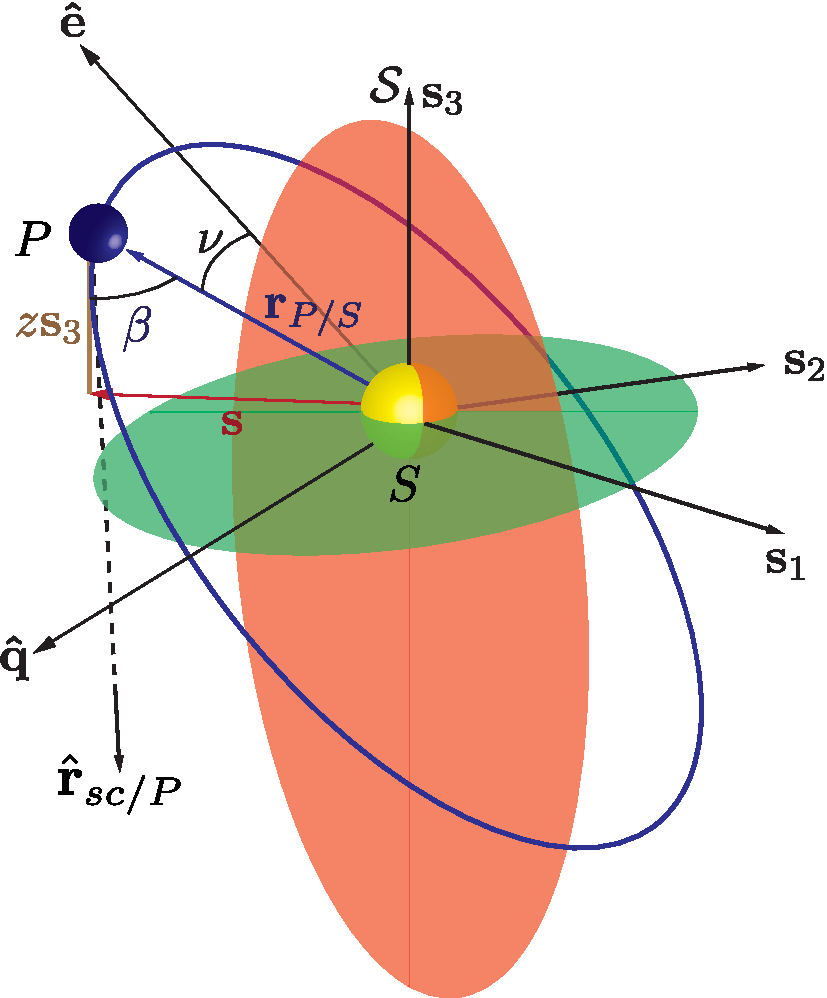
\includegraphics[width=0.6\textwidth]{orbit_diagram}
        \end{tabular}
    \end{center}
    \caption{\label{fig:orbit_diagram} Definition of reference frames and coordinates of simulated exosystems.  The observer lies along the negative $\mf s_3$ axis so that the observer-star unit vector is $+\mf s_3$.}
\end{figure}

The coordinate system of the simulated exosystems is defined as in \reffig{fig:orbit_diagram}.  The observer looks at the target star along the $\mathbf{s}_3$ axis, located at a distance $-d\mathbf{s}$ from the target at the time of observation. The argument of periapse, inclination,  and longitude of the ascending node ($\omega, I, \Omega$) are defined as a 3-1-3 rotation about the unit vectors defining the $\mathcal{S}$ reference frame.  This rotation defines the standard Equinoctial reference frame ($\mfhat{e}, \mfhat{q}, \mfhat{h}$), with the true anomaly ($\nu$) measured from $\mfhat{e}$).  The planet-star orbital radius vector $\mf r_{P/S}$ is projected into the $\mf s_1, \mf s_2$ plane as the projected separation vector $\mf s$, with magnitude $s$, and the phase (star-planet-observer) angle ($\beta$) is closely approximated by the angle between $\mf r_{P/s}$ and its projection onto $\mf s_3$.

The Planet Population module does not model the physics of planetary orbits or the amount of light reflected or emitted by a given planet, but rather encodes the statistics of planetary occurrence and properties. 

\label{sec:planetpopulation}
\subsubsection{Planet Population Object Attribute Initialization} 

\subsubsection*{Input}
The following are all entries in the passed specs dictionary (derived from the JSON script file or another dictionary).  Values not specified will be replaced with defaults, as listed.  It is important to note that many of these (in particular mass and radius) may be mutually dependent, and so some implementation may choose to only use some for inputs and set the rest via the physical models.

\begin{itemize}
\item
\begin{description}
    \item[arange (float 1$\times$2 array)] \hfill \\ Semi-major axis range in units of $ AU $. Default value is [0.01, 100]
    \item[erange (float 1$\times$2 array)] \hfill \\ Eccentricity range.  Default value is [0.01,0.99]
    \item[Irange (float 1$\times$2 array)] \hfill \\ Inclination range in units of $ deg $.  Default value is [0,180]
    \item[Orange (float 1$\times$2 array)] \hfill \\ Ascension of the ascending node range in units of $ deg $.  Default value is [0,360]
    \item[wrange (float 1$\times$2 array)] \hfill \\ Perigee range in units of $ deg $.  Default value is [0,360]
    \item[prange (float 1$\times$2 array)] \hfill \\ Planetary geometric albedo range.  Default value is [0.1,0.6]
    \item[Rprange (float 1$\times$2 array)] \hfill \\ Planetary Radius in Earth radii.  Default value is [1, 30]
    \item[Mprange (float 1$\times$2 array)] \hfill \\ Planetary mass in Earth masses.  Default value is [1, 4131]
    \item [scaleOrbits (boolean)] \hfill \\ Boolean where True means planetary orbits are scaled by the square root of stellar luminosity. Default value is False.
    \item[constrainOrbits (boolean)] \hfill \\ Boolean where True means planetary orbits are constrained to never leave the semi-major axis range (arange). Default value is False.
    \item[eta (float)] \hfill \\ The average occurrence rate of planets per star for the entire population.  The expected number of planets generated per simulation is equal to the product of eta with the total number of targets.  Note that this is the expectation value \emph{only}---the actual number of planets generated in a given simulation may vary depending on the specific method of sampling the population.
\end{description}
\end{itemize}

\subsubsection*{Attributes}
\begin{itemize}
\item
\begin{description}
    \item[PlanetPhysicalModel (PlanetPhysicalModel module)] \hfill \\ PlanetPhysicalModel class object
    \item[arange (astropy Quantity 1$\times$2 array)] \hfill \\ Semi-major axis range defined as [a\_min, a\_max] in units of $ AU $
    \item[erange (float 1$\times$2 ndarray)] \hfill \\ Eccentricity range defined as [e\_min, e\_max]
    \item[Irange (astropy Quantity 1$\times$2 array)] \hfill \\ Planetary orbital inclination range defined as [I\_min, I\_max] in units of $ deg $
    \item[Orange (astropy Quantity 1$\times$2 array)] \hfill \\ Right ascension of the ascending node range defined as [O\_min, O\_max] in units of $ deg $
    \item[wrange (astropy Quantity 1$\times$2 array)] \hfill \\ Argument of perigee range defined as [w\_min, w\_max] in units of $ deg $
    \item[prange (float 1$\times$2 ndarray)] \hfill \\ Planetary geometric albedo range defined as [p\_min, p\_max]
    \item[Rprange (astropy Quantity 1$\times$2 array)] \hfill \\ Planetary radius range defined as [R\_min, R\_max] in units of $earthRad$
    \item[Mprange (astropy Quantity 1$\times$2 array)] \hfill \\ Planetary mass range defined as [Mp\_min, Mp\_max] in units of $earthMass$
    \item[rrange (astropy Quantity 1$\times$2 array)] \hfill \\ Planetary orbital radius range defined as [r\_min, r\_max] derived from PlanetPopulation.arange and PlanetPopulation.erange, in units of $ AU $
    \item [scaleOrbits (boolean)] \hfill \\ Boolean where True means planetary orbits are scaled by the square root of stellar luminosity.
    \item[constrainOribts (boolean)] \hfill \\ Boolean where True means planetary orbits are constrained to never leave the semi-major axis range (arange). If set to True, an additional method (\verb+gen_eccen_from_sma+) must be provided by the implementation---see below.
    \item[eta (float)] \hfill \\ The average occurrence rate of planets per star for the entire population.
    \item[uniform (float, callable)] \hfill \\ Uniform distribution over a given range.
    \item[logunif (float, callable)] \hfill \\ Log-uniform distribution over a given range.
\end{description}
\end{itemize}

\subsubsection{Planet Population Value Generators} \label{sec:pdfs}
For each of the parameters represented by the input attributes, the planet population object will provide a method that returns random values for the attributes, within the ranges specified by each attribute (so that, for example, there will be samples of semi-major axis corresponding to \verb+arange+, etc.).  Each of these methods will take a single input of the number of values to generate.  These methods will encode the probability density functions representing each parameter, and use either a rejection sampler or other (numpy or scipy) provided sampling method to generate random values.  All returned values will have the same type/default units as the attributes. 

In cases where values need to be sampled jointly (for example if you have a joint distribution of semi-major axis and planetary radius) then the sampling will be encoded in the \verb+gen_plan_params+ function.  In cases where there is a deterministic calculation of one parameter from another (as in mass calculated from radius) this will be provided separately in the Planet Physical module. Any non-standard distribution functions being sampled by one of these methods should be created as object attributes in the implementation constructor so that they are available to other modules.
\\\\
The methods are:
\begin{itemize}[leftmargin=1.5in,font={\ttfamily}]
    \item[\texttt gen\_plan\_params] Returns values of semi-major axis (in units of $ AU $), eccentricity, geometric albedo, and planetary radius (in units of $ earthRad $)
    \item[\texttt gen\_angles] Returns values of orbital inclination, longitude of the ascending node, and argument of perigee, all in units of $ deg $
    \item[\texttt gen\_mass] Returns planetary mass values in units of $earthMass$
    \item[\texttt dist\_sma] Provides the probability density function for the semi-major axis
    \item[\texttt dist\_eccen] Provides the probability density function for the eccentricity
    \item[\texttt dist\_eccen\_from\_sma] Provides the probability density function for the eccentricity given a value of semi-major axis. This function is used when \verb+constrainOrbits+ is set to \verb+True+.
    \item[\texttt dist\_albedo] Provides the probability density function for the albedo
    \item[\texttt dist\_radius] Provides the probability density function for the radius
    \item[\texttt dist\_mass] Provides the probability density function for the mass
\end{itemize}


% PLANET PHYSICAL MODEL 

\subsection{Planet Physical Model} \label{sec:planetphysicalmodel}
The Planet Physical Model module contains models of the light emitted or reflected by planets in the wavelength bands under investigation by the current mission simulation.  It takes as inputs the physical quantities sampled from the distributions in the Planet Population module and generates synthetic spectra (or band photometry, as appropriate).  The specific implementation of this module can vary greatly, and can be based on any of the many available planetary geometric albedo, spectra and phase curve models.  As required, this module also provides physical models relating dependent parameters that cannot be sampled independently (for example density models relating plant mass and radius).  While the specific methods will depend highly on the physical models being used, the prototype provides four stubs that will be commonly useful:

\begin{itemize}[leftmargin=2in,font={\ttfamily}]
    \item[\texttt calc\_albedo\_from\_sma] Calculate planetary geometric albedo as a function of the semi-major axis.
    \item[\texttt calc\_radius\_from\_mass] Calculate planetary radii from their masses.
    \item[\texttt calc\_mass\_from\_radius] Calculate planetary masses from their radii.
    \item[\texttt calc\_Phi] Calculate the value of the planet phase function given its phase angle. The prototype implementation uses the Lambert phase function.
    \item[\texttt calc\_Teff] Calcluate the effective planet temperature given the stellar luminosity, planet albedo and star-planet distance.
\end{itemize}


% OPTICAL SYSTEM

\subsection{Optical System}
The Optical System module contains all of the necessary information to describe the planet signal and the background noise, and calculate the integration time for a given observation.  This first requires encoding the design of the telescope such as the optics attenuation, the diameter of the entrance pupil and the fraction of it that is obscured (by spiders and secondary mirror). A description of the science instruments is also required, with detector details such as read noise, dark current, and readout cycle. The baseline is assumed to be an imager and a spectrograph. Finally, the Optical System must include the performance of every selected starlight suppression systems, whether it be an internal coronagraph or an external occulter. The Optical System module also contains all the mission observing modes. Each mode is defined by a combination of a science instrument and a starlight suppression system, operating in a given spectral window.

The starlight suppression system throughput and contrast - or residual intensity - can be encoded with angular separation and wavelength dependant definitions. Some specific Optical System modules may also require encoding the Point Spread Functions (PSF) for on- and off-axis sources. At the opposite level of complexity, the encoded portions of this module may be a description of all of the optical elements between the telescope aperture and the science camera, along with a method of propagating an input wavefront to the final image plane.  Intermediate implementations can include partial propagations, or collections of static PSFs representing the contributions of various system elements.  The encoding of the optical train will allow for the extraction of specific bulk parameters including the instrument inner working angle (IWA), outer working angle (OWA), and mean and max contrast and throughput.

By definition, the detection mode IWA correspond to the working angle at which integration times are calculated during the detection phase. This IWA must not be confused with the global IWA. There are 3 types of IWA/OWA:\\
1- Each coronagraph has its own IWA/OWA in arcsec defined at its operation wavelength.\\
2- Each observing mode has its own IWA/OWA, based on the coronagraph IWA/OWA and rescaled to the mode’s specific wavelength. For simple cases where no observing modes are specified, the detection IWA will simply correspond to the coronagraph IWA.\\
3- A global IWA/OWA can be specified for the whole telescope, to filter out targets during the initialization, thus before the mission starts. By defaults, the global IWA = minimum(mode\_IWAs) and global OWA = maximum(mode\_OWAs). However, the user can specify a global IWA that is very small or even zero to avoid filtering out targets during initialization, without affecting the detection IWA described above.

The input and output of the Optical System methods are depicted in \reffig{fig:opticalsysmodule}. The Optical System module has three methods used in simulation:
\begin{itemize}[leftmargin=2in,font={\ttfamily}]
    \item[\texttt Cp\_Cb\_Csp] Called by \verb+calc_intTime+ to calculate the electron count rates for planet signal, background noise, and speckle residuals (see \S\ref{sec:CpCbCsptask}).
    \item[\texttt calc\_intTime] Calculates the integration times for specific values of planet zodiacal noise, delta magnitude, and angular separation (see \S\ref{sec:calcintTimetask}).
    \item[\texttt calc\_minintTime] Calculates the minimum integration times for all the stars from the target list, using optimistic input parameters  (see \S\ref{sec:calcminintTimetask}).
    \item[\texttt calc\_dMag\_per\_intTime] Calculates achievable planet delta magnitude per integration time (see \S\ref{sec:calcdMagperintTime}).
    \item[\texttt ddMag\_dt] Calculates derivative of achievable delta mag per integration time (see \S\ref{sec:ddMagdt}).
\end{itemize}

\begin{figure}[ht]
    \begin{center}
        \begin{tabular}{c}
            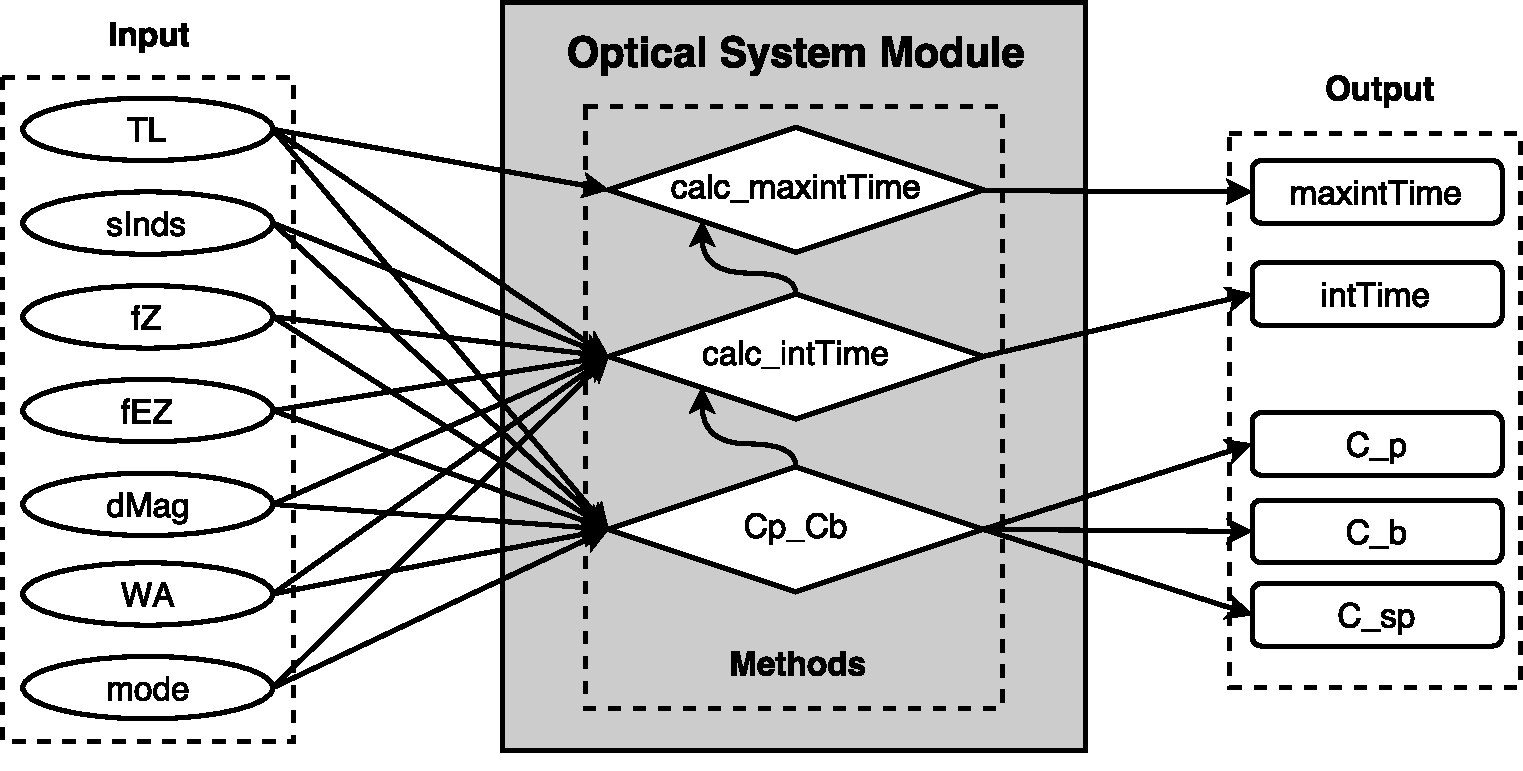
\includegraphics[width=\textwidth]{OpticalSystem}
        \end{tabular}
    \end{center}
    \caption{\label{fig:opticalsysmodule} Depiction of Optical System module methods including input and output (see \S\ref{sec:CpCbCsptask}, \S\ref{sec:calcintTimetask}).}
\end{figure}

\label{sec:opticalsystem}
\subsubsection{Optical System Object Attribute Initialization} 

The specific set of inputs to this module will vary based on the simulation approach used.  Here we define the specification for the case where static PSF(s), derived from external diffraction modeling, are used to describe the system.  Note that some of the inputs are specific to "internal" or "external" (i.e. starshade) systems and will be expected based on the $occulter$ flag.

\subsubsection*{Input}

\begin{itemize}
\item 
\begin{description}
    \item[obscurFac (float)] \hfill \\ Obscuration factor due to secondary mirror and spiders. Default value is 0.1.
    \item[shapeFac (float)] \hfill \\ Shape factor of the unobscured pupil area, so that $ shapeFac \times pupilDiam^2  \times (1-obscurFac) = pupilArea $. Default value is $ \frac{\pi}{4} $.
    \item[pupilDiam (float)] \hfill \\ Entrance pupil diameter in  $ m $. Default value is 4.
    \item[IWA (float)] \hfill \\ Fundamental Inner Working Angle in units of $ arcsec $. No planets can ever be observed at smaller separations. If not set, defaults to smallest IWA of all starlightSuppressionSystems.
    \item[OWA (float)] \hfill \\ Fundamental Outer Working Angle in units of $ arcsec $. Set to $ Inf $ for no OWA. If not set, defaults to largest OWA of all starlightSuppressionSystems. JSON values of 0 will be interpreted as $ Inf $.
    \item[intCutoff (float)] \hfill \\ Maximum allowed integration time in units of $ day $. No integration will be started that would take longer than this value. Default value is 50.
    \item[dMag0 (float)] \hfill \\  Favorable planet delta magnitude value used to calculate the minimum integration times for inclusion in target list.
    \item[WA0 (float)] \hfill \\  Instrument working angle value used to calculate the minimum integration times for inclusion in target list (defaults to detection IWA-OWA midpoint), in units of $arcsec$.
    \item[scienceInstruments (list of dicts)] \hfill\\ List of dictionaries containing specific attributes of all science instruments. For each instrument, if the below attributes are missing from the dictionary, they will be assigned the default values listed, or any value directly passed as input to the class constructor. 
    \begin{description}
        \item[name (string)] \hfill\\ (Required) Instrument name (e.g. imager-EMCCD, spectro-CCD), should contain the type of instrument (imager or spectro). Every instrument should have a unique name.
        \item[QE (float, callable)] \hfill \\ Detector quantum efficiency: either a scalar for constant QE, or a two-column array for wavelength-dependent QE, where the first column contains the wavelengths in units of $ nm $. May be data or FITS filename. Default is scalar 0.9. 
        \item[optics (float)] \hfill \\ Attenuation due to optics specific to the science instrument. Default value is 0.5.
        \item[FoV (float)] \hfill \\ Field of view in units of $ arcsec $. Default value is 10.
        \item[pixelNumber (integer)] \hfill \\ Detector array format, number of pixels per detector lines/columns. Default value is 1000.
        \item[pixelSize (float)] \hfill \\ Pixel pitch in units of $ m $. Default value is 1e-5. 
        \item[sread (float)] \hfill \\ Detector effective read noise per frame per pixel, including any gain (e.g. electron multiplication gain). Default value is 1e-6.
        \item[idark (float)] \hfill \\ Detector dark-current per pixel in units of $ 1/s $. Default value is 1e-4. 
        \item[CIC (float)] \hfill \\ (Specific to CCDs) Clock-induced-charge per frame per pixel. Default value is 1e-3. 
        \item[texp (float)] \hfill \\ Exposure time per frame in units of $ s $. Default value is 100. 
        \item[radDos (float)] \hfill \\ Radiation dosage. Default value is 0.
        \item[PCeff (float)] \hfill \\ Photon counting efficiency. Default value is 0.8.
        \item[ENF (float)] \hfill \\ (Specific to EM-CCDs) Excess noise factor. Default value is 1.
        \item[Rs (float)] \hfill \\ (Specific to spectrometers) Spectral resolving power defined as $\lambda/d\lambda$. Default value is 50. 
        \item[lenslSamp (float)] \hfill \\ (Specific to spectrometers) Lenslet sampling, number of pixel per lenslet rows or cols. Default value is 2.
    \end{description}
    \item[starlightSuppressionSystems (list of dicts)] \hfill\\ List of dictionaries containing specific attributes of all starlight suppression systems. For each system, if the below attributes are missing from the dictionary, they will be assigned the default values listed, or any value directly passed as input to the class constructor. In case of multiple systems, specified wavelength values (lam, deltaLam, BW) of the first system become the new default values.
    
    The following items can be encoded either as scalar parameters, or as two-column arrays for angular separation-dependent parameters, where the first column contains the separations in units of $ arcsec $, or as 2D array for angular separation- and wavelength- dependent parameters, where the first column contains the angular separation values in units of $ arcsec $ and the first row contains the wavelengths in units of $ nm $: $occ\_trans$, $core\_thruput$, $core\_contrast$, $core\_mean\_intensity$, $core\_area$. 
    \begin{description}
        \item[name (string)] \hfill \\ (Required) System name (e.g. HLC-500, SPC-700), should also contain the central wavelength the system is optimized for. Every system must have a unique Name. 
        \item[optics (float)] \hfill \\ Attenuation due to optics specific to the coronagraph, e.g. polarizer, Lyot stop, extra flat mirror. Default value is 1.
        \item[lam (float)] \hfill \\ Central wavelength $\lambda$ in units of $ nm $. Default value is 500. 
        \item[deltaLam (float)] \hfill \\ Bandwidth $ \Delta\lambda $ in units of $ nm $. Defaults to lambda $ \times $ BW (defined hereunder).
        \item[BW (float)] \hfill \\ Bandwidth fraction $(\Delta\lambda/\lambda)$. Only applies when deltaLam is not specified. Default value is 0.2.
        \item[IWA (float)] \hfill \\ Inner Working Angle of this system in units of $ arcsec $. If not set, or if too small for this system contrast/throughput definitions, defaults to smallest WA of contrast/throughput definitions.
        \item[OWA (float)] \hfill \\ Specific Outer Working Angle of this system in units of $ arcsec $. Set to $ Inf $ for no OWA. If not set, or if too large for this system contrast/throughput definitions, defaults to largest WA of contrast/throughput definitions.  JSON values of $ 0 $ will be interpreted as $ Inf $.
        \item[occ\_trans (float, callable)] \hfill \\ Intensity transmission of extended background sources such as zodiacal light. Includes pupil mask, occulter, Lyot stop and polarizer. Default is scalar 0.2.
        \item[core\_thruput (float, callable)] \hfill \\ System throughput in the FWHM region of the planet PSF core. Default is scalar 0.1.
        \item[core\_contrast (float, callable)] \hfill \\ System contrast defined as the starlight residual normalized intensity in the PSF core, divided by the core throughput. Default is scalar 1e-10.
        \item[core\_mean\_intensity (float, callable)] \hfill \\ Mean starlight residual normalized intensity per pixel, required to calculate the total core intensity as $core\_mean\_intensity \times Npix$. If not specified, then the total core intensity is equal to $core\_contrast \times core\_thruput$.
        \item[core\_area (float, callable)] \hfill \\ Area of the FWHM region of the planet PSF, in units of $ arcsec^2 $. If not specified, the default core area is equal to $\pi\left(\frac{\sqrt 2}{2}\frac{\lambda}{D}\right)^2$.
        \item[core\_platescale (float)] \hfill \\ Platescale used for a specific set of coronagraph parameters, in units of lambda/D per pixel. Defaults to the instrument pixelScale.
        \item[ohTime (float)] \hfill \\ Optical system overhead time in units of $ day $.  Default value is 1.  This is the (assumed constant) amount of time required to set up the optical system (i.e., dig the dark hole or do fine alignment with the occulter).  It is added to every observation, and is separate from the observatory overhead defined in the observatory module, which represents the observatory's settling time.  Both overheads are added to the integration time to determine the full duration of each detection observation.
        \item[occulter (boolean)] \hfill \\ True if the system has an occulter (external or hybrid system), otherwise False (internal system)
        \item[occulterDiameter (float)]\hfill \\ Occulter diameter in units of $ m $.  Measured petal tip-to-tip.
        \item [NocculterDistances (integer)]\hfill \\ Number of telescope separations the occulter operates over (number of occulter bands). If greater than 1, then the occulter description is an array of dicts.
        \item[occulterDistance (float)] \hfill \\ Telescope-occulter separation in units of $km$.
        \item[occulterBlueEdge (float)]\hfill \\ Occulter blue end of wavelength band in units of $nm$.
        \item[occulterRedEdge (float)]\hfill \\ Occulter red end of wavelength band in units of $nm$.
    \end{description}
    \item[observingModes (list of dicts)]\hfill \\ List of dictionaries containing specific attributes of all mission observing modes. Each observing mode is a combination of an instrument and a system, operating at a given wavelength, which by default is the wavelength defined in the starlight suppression system of the observing mode. If an observing mode is operating at a different wavelength than the system default wavelength, then this new wavelength must be added to the observing mode, and the system performance will be automatically rescaled to the new wavelength. If no observing mode is defined, the default observing mode simply combines the first instrument and the first system.
    
    \begin{description}
        \item[instName (string)]\hfill \\ (Required) Instrument name. Must match with the name of a defined science instrument.
        \item[systName (string)]\hfill \\ (Required) System name. Must match with the name of a defined starlight suppression system.
        \item[inst (dict)]\hfill \\ Selected instrument of the observing mode.
        \item[syst (dict)]\hfill \\ Selected system of the observing mode.
        \item[detectionMode (boolean)]\hfill \\ True if this observing mode is the detection mode, otherwise False. Only one detection mode can be specified. If not specified, default detection mode is first imager mode.
        \item[SNR (float)]\hfill \\ Signal-to-noise ratio threshold. Defaults to 5.
        \item[timeMultiplier (float)]\hfill \\ Integration time multiplier. Equal to the number of discrete integrations needed to cover the full field of view (e.g. shaped pupil), or the full wavelength band and all required polarization states.  For example, if the band is split into three sub-bands, and there are two polarization states that must be measured, and each of these must be done sequentially, then this value would equal 6.  However, if the three sub-bands could be observed at the same time (e.g., by separate detectors) then the value would be two (for the two polarization states). Defaults to 1.
        \item[lam (float)]\hfill \\ Central wavelength in units of nm. Defaults to corresponding system value.
        \item[deltaLam (float)]\hfill \\ Bandwidth in units of nm. Defaults to corresponding system value.
        \item[BW (float)]\hfill \\ Bandwidth fraction. Defaults to corresponding system value.
    \end{description}
\end{description}
\end{itemize}
For all values that may be either scalars or interpolants, in the case where scalar values are given, the optical system module will automatically wrap them in lambda functions so that they become callable (just like the interpolant) but will always return the same value for all arguments.  The inputs for interpolants may be filenames (full absolute paths) with tabulated data, or NumPy ndarrays of argument and data (in that order in rows so that input[0] is the argument and input[1] is the data).  When the input is derived from a JSON file, these must either be scalars or filenames.

The starlight suppression system and science instrument dictionaries can contain any other attributes required by a particular optical system implementation.  The only significance of the ones enumerated above is that they are explicitly checked for by the prototype constructor, and cast to their expected values.

\subsubsection*{Attributes}
These will always be present in an OpticalSystem object and directly accessible as \verb+OpticalSystem.Attribute+.
\begin{itemize}
\item 
\begin{description}
    \item[obscurFac (float)] \hfill \\ Obscuration factor due to secondary mirror and spiders
    \item[shapeFac (float)] \hfill \\ Shape factor of the unobscured pupil area, so that $ shapeFac \times pupilDiam^2  \times (1-obscurFac) = pupilArea $
    \item[pupilDiam (astropy Quantity)] \hfill \\ Entrance pupil diameter in units of $ m $
    \item[pupilArea (astropy Quantity)] \hfill \\ Entrance pupil area in units of $ m^{2} $
    \item[haveOcculter (boolean)] \hfill \\ Boolean signifying if the system has an occulter
    \item[IWA (astropy Quantity)] \hfill \\ Fundamental Inner Working Angle in units of $ arcsec $
    \item[OWA (astropy Quantity)] \hfill \\ Fundamental Outer Working Angle in units of $ arcsec $
    \item[intCutoff (astropy Quantity)] \hfill \\ Maximum allowed integration time in units of $ day $
    \item[dMag0 (float)] \hfill \\  Favorable planet delta magnitude value used to calculate the minimum integration times for inclusion in target list.
    \item[WA0 (astropy Quantity)] \hfill \\  Instrument working angle value used to calculate the minimum integration times for inclusion in target list.
    \item[scienceInstruments (list of dicts)] \hfill \\  List of dictionaries containing all supplied science instrument attributes.  Typically the first instrument will be the imager, and the second the spectrograph (IFS). Only required attribute is `name'.  See above for other commonly used attributes. 
    \item[starlightSuppressionSystems (list of dicts)] \hfill \\  List of dictionaries containing all supplied starlight suppression system attributes. Typically the first system will be used with the imager, and the second with the IFS. Only required attribute is `name'. See above for other commonly used attributes.
    \item[observingModes (list of dicts)] \hfill \\  List of dictionaries containing all mission observing modes. Only required attribute are `instName' and `systName'. See above for other commonly used attributes.
\end{description}
\end{itemize}

\subsubsection{Cp\_Cb\_Csp Method} \label{sec:CpCbCsptask}
The \verb+Cp_Cb_Csp+ method calculates the electron count rates for planet signal, background noise, and speckle residuals.

\subsubsection*{Input}
\begin{itemize}
\item 
    \begin{description}
    \item[TL (TargetList module)] \hfill \\ TargetList class object, see \S\ref{sec:targetlist} for definition of available attributes
    \item[sInds (integer ndarray)] \hfill \\ Integer indices of the stars of interest
    \item[fZ (astropy Quantity array)] \hfill \\ Surface brightness of local zodiacal light in units of $ 1/arcsec^2 $
    \item[fEZ (astropy Quantity array)] \hfill \\ Surface brightness of exo-zodiacal light in units of $ 1/arcsec^2 $
    \item[dMag (float ndarray)] \hfill \\ Differences in magnitude between planets and their host star.
    \item[WA (astropy Quantity array)] \hfill \\ Working angles of the planets of interest in units of $arcsec$
    \item[mode (dict)] \hfill \\ Selected observing mode
\end{description}
\end{itemize}

\subsubsection*{Output}
\begin{itemize}
\item 
\begin{description}
    \item[C\_p (astropy Quantity array)] \hfill \\ Planet signal electron count rate in units of $ 1/s $
    \item[C\_b (astropy Quantity array)] \hfill \\ Background noise electron count rate in units of $ 1/s $
    \item[C\_sp (astropy Quantity array)] \hfill \\ Residual speckle spatial structure (systematic error) in units of $ 1/s $
\end{description}
\end{itemize}

\subsubsection{calc\_intTime Method} \label{sec:calcintTimetask}
The \verb+calc_intTime+ method calculates the integration time required for specific planets of interest.  This method is called from the SurveySimulation module.

\subsubsection*{Input}
\begin{itemize}
\item 
\begin{description}
    \item[TL (TargetList module)] \hfill \\ TargetList class object, see \S\ref{sec:targetlist} for definition of available attributes
    \item[sInds (integer ndarray)] \hfill \\ Integer indices of the stars of interest
    \item[fZ (astropy Quantity array)] \hfill \\ Surface brightness of local zodiacal light in units of $ 1/arcsec^2 $
    \item[fEZ (astropy Quantity array)] \hfill \\ Surface brightness of exo-zodiacal light in units of $ 1/arcsec^2 $
    \item[dMag (float ndarray)] \hfill \\ Differences in magnitude between planets and their host star.
    \item[WA (astropy Quantity array)] \hfill \\ Working angles of the planets of interest in units of $ arcsec $
    \item[mode (dict)] \hfill \\ Selected observing mode
\end{description}
\end{itemize}

\subsubsection*{Output}
\begin{itemize}
\item 
\begin{description}
    \item[intTime (astropy Quantity array)] \hfill \\ Integration time for each of the planets of interest in units of $ day $
\end{description}
\end{itemize}


\subsubsection{calc\_minintTime Method} \label{sec:calcminintTimetask}
The \verb+calc_minintTime+ method calculates the minimum integration time for each star in the target list.  This method is called from the TargetList module.

\subsubsection*{Input}
\begin{itemize}
\item 
\begin{description}
    \item[TL (TargetList module)] \hfill \\ TargetList class object, see \S\ref{sec:targetlist} for definition of available attributes
\end{description}
\end{itemize}

\subsubsection*{Output}
\begin{itemize}
\item
\begin{description}
    \item[minintTime (astropy Quantity array)] \hfill \\ Minimum integration time for each target star in units of $ day $
\end{description}
\end{itemize}


\subsubsection{calc\_dMag\_per\_intTime Method} \label{sec:calcdMagperintTime}
The \verb+calc_dMag_per_intTime+ method calculates the achievable planet delta magnitude (delta mag) for one integration time per star in the input list at one or more working angles.

\subsubsection*{Input}
\begin{itemize}
\item 
\begin{description}
    \item[intTime (astropy Quantity array)] \hfill \\ Integration times in units of $ day $
    \item[TL (TargetList module)] \hfill \\ TargetList class object, see \S\ref{sec:targetlist} for definition of available attributes
    \item[sInds (integer ndarray)] \hfill \\ Integer indices of the stars of interest
    \item[fZ (astropy Quantity array)] \hfill \\ Surface brightness of local zodiacal light in units of $ 1/arcsec^2 $
    \item[fEZ (astropy Quantity array)] \hfill \\ Surface brightness of exo-zodiacal light in units of $ 1/arcsec^2 $
    \item[WA (astropy Quantity array)] \hfill \\ Working angles of the planets of interest in units of $ arcsec $
    \item[mode (dict)] \hfill \\ Selected observing mode
\end{description}
\end{itemize}

\subsubsection*{Output}
\begin{itemize}
\item 
\begin{description}
    \item[dMag (float ndarray)] \hfill \\ Achievable dMag for given integration time and working angle
\end{description}
\end{itemize}


\subsubsection{ddMag\_dt Method} \label{sec:ddMagdt}
The \verb+ddMag_dt+ method calculates the derivative of achievable dMag with respect to integration time.

\subsubsection*{Input}
\begin{itemize}
\item 
\begin{description}
    \item[intTime (astropy Quantity array)] \hfill \\ Integration times in units of $ day $
    \item[TL (TargetList module)] \hfill \\ TargetList class object, see \S\ref{sec:targetlist} for definition of available attributes
    \item[sInds (integer ndarray)] \hfill \\ Integer indices of the stars of interest
    \item[fZ (astropy Quantity array)] \hfill \\ Surface brightness of local zodiacal light in units of $ 1/arcsec^2 $
    \item[fEZ (astropy Quantity array)] \hfill \\ Surface brightness of exo-zodiacal light in units of $ 1/arcsec^2 $
    \item[WA (astropy Quantity array)] \hfill \\ Working angles of the planets of interest in units of $ arcsec $
    \item[mode (dict)] \hfill \\ Selected observing mode
\end{description}
\end{itemize}

\subsubsection*{Output}
\begin{itemize}
\item 
\begin{description}
    \item[ddMagdt (astropy Quantity array)] \hfill \\ Derivative of achievable dMag with respect to integration time in units of $ 1/s $
\end{description}
\end{itemize}


% ZODIACAL LIGHT 

\subsection{Zodiacal Light}\label{sec:zodiacallight}

The input and output of the Zodiacal Light methods are depicted in \reffig{fig:zodiacallightmodule}. The Zodiacal Light module contains two methods:
\begin{itemize}[leftmargin=1in,font={\ttfamily}]
    \item[\texttt fZ] Calculates the surface brightness of local zodiacal light  (see \S\ref{sec:fZtask})
    \item[\texttt fEZ] Calculates the surface brightness of exozodiacal light (see \S\ref{sec:fEZtask})
\end{itemize}

\begin{figure}[ht]
    \begin{center}
        \begin{tabular}{c}
             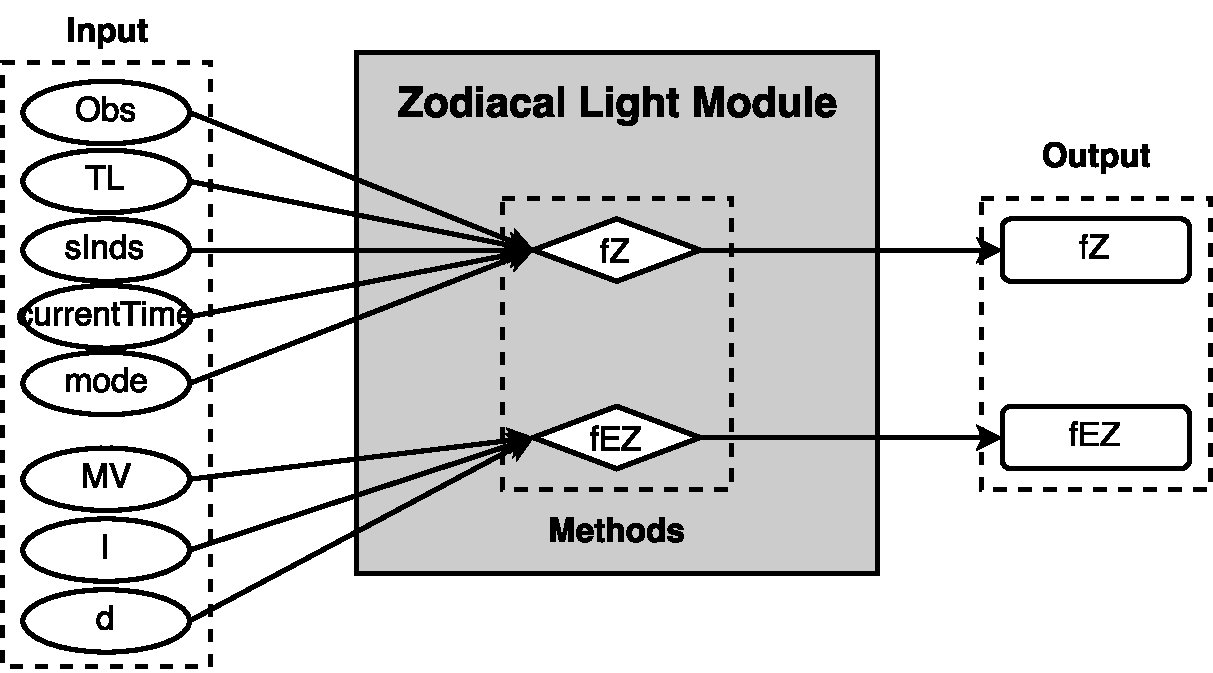
\includegraphics[width=0.8\textwidth]{ZodiTasks2}
        \end{tabular}
    \end{center}
    \caption{\label{fig:zodiacallightmodule} Depiction of Zodiacal Light module methods including input and output (see \S\ref{sec:fZtask} and \S\ref{sec:fEZtask}).}
\end{figure}

\subsubsection{Zodiacal Light Object Attribute Initialization}

\subsubsection*{Input}
\begin{itemize}
\item
\begin{description}
    \item[magZ (float)] \hfill \\ Zodiacal light brightness magnitude (per $ arcsec^2 $). Defaults to 23.
    \item[magEZ (float)] \hfill \\ Exo-zodiacal light brightness magnitude (per $ arcsec^2 $). Defaults to 22.
    \item[varEZ (float)] \hfill \\ Exo-zodiacal light variation (variance of log-normal distribution). Defaults to 0 (constant exo-zodiacal light).
\end{description}
\end{itemize}

\subsubsection*{Attributes}
\begin{itemize}
\item
\begin{description}
    \item[magZ (float)] \hfill \\ Zodi brightness magnitude (per $ arcsec^2 $)
    \item[magEZ (float)] \hfill \\ Exo-zodi brightness magnitude (per $ arcsec^2 $)
    \item[varEZ (float)] \hfill \\ Exo-zodiacal light variation (variance of log-normal distribution)
    \item[fZ0 (astropy Quantity)] \hfill \\ Default surface brightness of zodiacal light in units of $ 1/arcsec^2 $ 
    \item[fEZ0 (astropy Quantity)] \hfill \\ Default surface brightness of exo-zodiacal light in units of $ 1/arcsec^2 $ 
\end{description}
\end{itemize}

\subsubsection{fZ Method} \label{sec:fZtask}
The \verb+fZ+ method returns surface brightness of local zodiacal light for planetary systems.  This functionality is used by the Simulated Universe module.

\subsubsection*{Input}
\begin{itemize}
\item 
\begin{description}
    \item[Obs (Observatory module)] \hfill \\ Observatory class object, see \S\ref{sec:observatory} for description of functionality and attributes       
    \item[TL (TargetList module)] \hfill \\ TargetList class object, see \S\ref{sec:targetlist} for description of functionality and attributes       
    \item[sInds (integer ndarray)] \hfill \\ Integer indices of the stars of interest
    \item[currentTime (astropy \href{http://astropy.readthedocs.org/en/latest/time/index.html}{Time} array)] \hfill \\ Current absolute mission time in MJD    
    \item[mode (dict)] \hfill \\ Selected observing mode
\end{description}
\end{itemize}

\subsubsection*{Output}
\begin{itemize}
\item 
\begin{description}
    \item[fZ (astropy Quantity array)] \hfill \\ Surface brightness of zodiacal light in units of $ 1/arcsec^2 $
\end{description}
\end{itemize}

\subsubsection{fEZ Method} \label{sec:fEZtask}
The \verb+fEZ+ method returns surface brightness of exo-zodiacal light for planetary systems.  This functionality is used by the Simulated Universe module.

\subsubsection*{Input}
\begin{itemize}
\item 
\begin{description}
    \item[MV (integer ndarray)] \hfill \\ Apparent magnitude of the star (in the V band)
    \item[I (astropy Quantity array)] \hfill \\ Inclination of the planets of interest in units of $ deg $
    \item[d (astropy Quantity n$\times$3 array)] \hfill \\ Distance to star of the planets of interest in units of $AU$
\end{description}
\end{itemize}

\subsubsection*{Output}
\begin{itemize}
\item 
\begin{description}
    \item[fEZ (astropy Quantity array)] \hfill \\ Surface brightness of exo-zodiacal light in units of $ 1/arcsec^2 $
\end{description}
\end{itemize}


% BACKGROUND SOURCES

\subsection{Background Sources}\label{sec:backgroundsources}

The Background Sources module provides density of background sources for a given target based on its coordinates and the integration depth. The integration depth is the limiting planet magnitude, that is the magnitude of the faintest planet we can observe. This will be used in the post-processing module to determine false alarms based on confusion.  The prototype module has no inputs and only a single function: \verb+dNbackground+ (see \S\ref{sec:dNbackgroundtask}).

\subsubsection{dNbackground Method} \label{sec:dNbackgroundtask}

\subsubsection*{Input}
\begin{itemize}
\item 
\begin{description}
    \item[coords (astropy SkyCoord array)] \hfill \\ \href{http://astropy.readthedocs.org/en/latest/api/astropy.coordinates.SkyCoord.html}{SkyCoord object} containing right ascension, declination, and  distance to star of the planets of interest in units of $ deg $, $ deg $ and $ pc $.
    \item[intDepths (float ndarray)] \hfill \\ Integration depths equal to the planet magnitude (Vmag+dMag), i.e. the V magnitude of the dark hole to be produced for each target. Must be of same length as coords.
\end{description}
\end{itemize}

\subsubsection*{Output}
\begin{itemize}
\item 
\begin{description}
    \item[dN (astropy Quantity array)] \hfill \\ Number densities of background sources for given targets in  units of $ 1/arcmin^2 $. Same length as inputs.
\end{description}
\end{itemize}


% POST-PROCESSING

\subsection{Post-Processing}\label{sec:postprocessing}
The Post-Processing module encodes the effects of post-processing on the data gathered in a simulated observation, and the effects on the final contrast of the simulation.  The Post-Processing module is also responsible for determining whether a planet detection has occurred for a given observation, returning one of four possible states---true positive (real detection), false positive (false alarm), true negative (no detection when no planet is present) and false negative (missed detection).  These can be generated based solely on statistical modeling or by processing simulated images.

The Post-Processing module contains the \verb+det_occur+ method (see \S\ref{sec:detoccurtask}).  This method determines if a planet detection occurs for a given observation.  The input and output of this method are depicted in \reffig{fig:postprocessingmodule}.

\begin{figure}[ht]
    \begin{center}
        \begin{tabular}{c}
            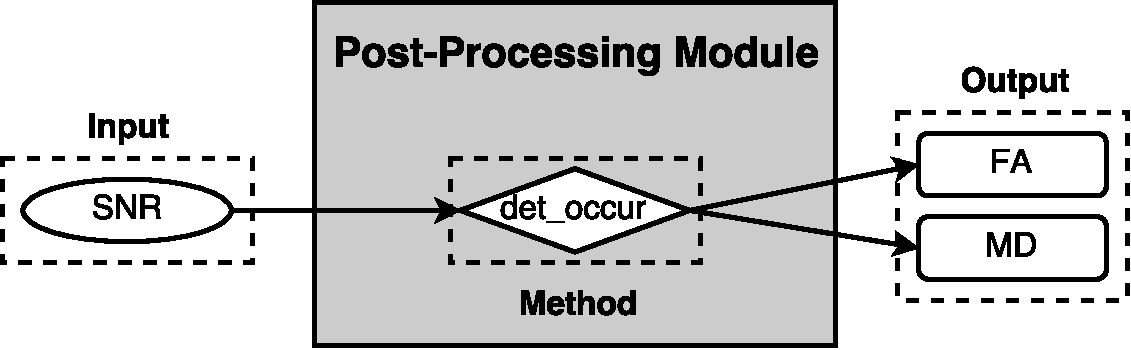
\includegraphics[width=0.8\textwidth]{PostProcessing2}
        \end{tabular}
    \end{center}
    \caption{\label{fig:postprocessingmodule} Depiction of Post-Processing module method including input and output (see \S\ref{sec:detoccurtask}).}
\end{figure}

\subsubsection{Post-Processing Object Attribute Initialization}

\subsubsection*{Input}
\begin{itemize}
\item 
\begin{description}
    \item[FAP (float)] \hfill \\ Detection false alarm probability. Default value is $3 \times 10^{-7}$.
    \item[MDP (float)] \hfill \\ Missed detection probability. Default value is $10^{-3}$.
    \item[ppFact (float, callable)] \hfill \\ Post-processing contrast factor, between 0 and 1: either a scalar for constant gain, or a two-column array for separation-dependent gain, where the first column contains the angular separation in units of $arcsec$. May be data or FITS filename. Default value is 1.
    \item[FAdMag0 (float, callable)] \hfill \\ Minimum delta magnitude that can be obtained by a false alarm: either a scalar for constant dMag, or a two-column array for separation-dependent dMag, where the first column contains the angular separation in units of arcsec. May be data or FITS filename. Default value is 15.
\end{description}
\end{itemize}

\subsubsection*{Attributes}
\begin{itemize}
\item 
\begin{description}
    \item[BackgroundSources (BackgroundSources module)] \hfill \\
        BackgroundSources class object (see \ref{sec:backgroundsources})
    \item[FAP (float)] \hfill \\ Detection false alarm probability
    \item[MDP (float)] \hfill \\ Missed detection probability
    \item[ppFact (float, callable)] \hfill \\ Post-processing contrast factor, between 0 and 1.
    \item[FAdMag0 (float, callable)] \hfill \\ Minimum delta magnitude that can be obtained by a false alarm.
\end{description}
\end{itemize}

\subsubsection{det\_occur Method} \label{sec:detoccurtask}
The \verb+det_occur+ method determines if a planet detection has occurred.

\subsubsection*{Input}
\begin{itemize}
\item 
\begin{description}
    \item[SNR (float ndarray)] \hfill \\ Signal-to-noise ratio of the planets around the selected target
    \item[mode (dict)] \hfill \\ Selected observing mode
    \item[TL (TargetList module)] \hfill \\ TargetList class object
    \item[sInd (integer)] \hfill \\ Index of the star being observed
    \item[intTime (astropy Quantity)] \hfill \\ Selected star integration time for detection
\end{description}
\end{itemize}

\subsubsection*{Output}
\begin{itemize}
\item 
\begin{description}
    \item[FA (boolean)] \hfill \\ False alarm (false positive) boolean.
    \item[MD (boolean ndarray)] \hfill \\ Missed detection (false negative) boolean with the size of number of planets around the target.
\end{description}
\end{itemize}


% COMPLETENESS

\subsection{Completeness}\label{sec:completeness}
The Completeness module takes in information from the Planet Population module to determine initial completeness and update completeness values for target list stars when called upon.

The Completeness module contains the following methods:
\begin{itemize}[leftmargin=2in,font={\ttfamily}]
    \item[\texttt target\_completeness] Generates initial completeness values for each star in the target list (see \S\ref{sec:targetcompletenesstask})
    \item[\texttt gen\_update] generates dynamic completeness values for successive observations of each star in the target list  (see \S\ref{sec:genupdatetask})
    \item[\texttt completeness\_update] Updates the completeness values following an observation (see \S\ref{sec:completenessupdatetask})
    \item[\texttt comp\_per\_intTime] Calculates completeness values per integration time (see \S\ref{sec:compperintTime}) 
    \item[\texttt dcomp\_dt] Calculates derivative of completeness with respect to integration time (see \S\ref{sec:dcompdt})
\end{itemize}

\subsubsection{Completeness Object Attribute Initialization}

\subsubsection*{Input}
\begin{itemize}
\item 
\begin{description}
    \item[dMagLim (float)] \hfill \\ Limiting planet-to-star delta magnitude for completeness. Defaults to 25.
    \item[minComp (float)] \hfill \\ Minimum completeness value for inclusion in target list.  Defaults to 0.1.
\end{description}
\end{itemize}
Monte Carlo methods for calculating completeness will require an input of the number of planet samples called \verb+Nplanets+. 

\subsubsection*{Attributes}
\begin{itemize}
\item 
\begin{description}
    \item[PlanetPopulation (PlanetPopulation module)] \hfill \\ PlanetPopulation object (see \ref{sec:planetpopulation})
    \item[PlanetPhysicalModel (PlanetPhysicalModel module)] \hfill \\ PlanetPhysicalModel module object (see \ref{sec:planetphysicalmodel}) 
    \item[dMagLim (float)] \hfill \\ Limiting planet-to-star delta magnitude for completeness
    \item[minComp (float)] \hfill \\ Minimum completeness value for inclusion in target list
\end{description}
\end{itemize}

\subsubsection{target\_completeness Method}
\label{sec:targetcompletenesstask}
The \verb+target_completeness+ method generates completeness values for each star in the target list.

\subsubsection*{Input}
\begin{itemize}
\item 
\begin{description}
    \item[TL (TargetList module)] \hfill \\ TargetList class object, see \S\ref{sec:targetlist} for definition of functionality and attributes
\end{description}
\end{itemize}

\subsubsection*{Output}
\begin{itemize}
\item 
\begin{description}
    \item[comp0 (float ndarray)] \hfill \\ Contains completeness values for each star in the target list
\end{description}
\end{itemize}

\subsubsection{gen\_update Method} \label{sec:genupdatetask}
The \verb+gen_update+ method generates dynamic completeness values for successive observations of each star in the target list.

\subsubsection*{Input}
\begin{itemize}
\item 
\begin{description}
    \item[TL (TargetList module)] \hfill \\ TargetList class object, see \S\ref{sec:targetlist} for definition of functionality and attributes
\end{description}
\end{itemize}

\subsubsection{completeness\_update Method}
\label{sec:completenessupdatetask}
The \verb+completeness_update+ method updates the completeness values for each star in the target list following an observation.

\subsubsection*{Input}
\begin{itemize}
\item 
\begin{description}
    \item[TL (TargetList module)] \hfill \\ TargetList class object, see \S\ref{sec:targetlist} for definition of functionality and attributes
    \item[sInds (integer array)] \hfill \\ Indices of stars to update
    \item[visits (integer array)] \hfill \\ Number of visits for each star
    \item[dt (astropy Quantity array)] \hfill \\ Time since previous observation
\end{description}
\end{itemize}

\subsubsection*{Output}
\begin{itemize}
\item 
\begin{description}
    \item[comp0 (float ndarray)] \hfill \\
        Updated completeness values for each star in the target list
\end{description}
\end{itemize}

\subsubsection{comp\_per\_intTime Method}
\label{sec:compperintTime}
The \verb+comp_per_intTime+ method calculates the completeness values per integration time.

\subsubsection*{Input}
\begin{itemize}
\item 
\begin{description}
    \item[intTime (astropy Quantity array)] \hfill \\ Integration times in units of $ day $
    \item[TL (TargetList module)] \hfill \\ TargetList class object, see \S\ref{sec:targetlist} for definition of available attributes
    \item[sInds (integer ndarray)] \hfill \\ Integer indices of the stars of interest
    \item[fZ (astropy Quantity array)] \hfill \\ Surface brightness of local zodiacal light in units of $ 1/arcsec^2 $
    \item[fEZ (astropy Quantity array)] \hfill \\ Surface brightness of exo-zodiacal light in units of $ 1/arcsec^2 $
    \item[WA (astropy Quantity array)] \hfill \\ Working angles of the planets of interest in units of $ arcsec $
    \item[mode (dict)] \hfill \\ Selected observing mode
\end{description}
\end{itemize}

\subsubsection*{Output}
\begin{itemize}
\item 
\begin{description}
    \item[comp (float ndarray)] \hfill \\
        Completeness values
\end{description}
\end{itemize}

\subsubsection{dcomp\_dt Method}
\label{sec:dcompdt}
The \verb+dcomp_dt+ method calculates the derivative of completeness with respect to integration time.

\subsubsection*{Input}
\begin{itemize}
\item 
\begin{description}
    \item[intTime (astropy Quantity array)] \hfill \\ Integration times in units of $ day $
    \item[TL (TargetList module)] \hfill \\ TargetList class object, see \S\ref{sec:targetlist} for definition of available attributes
    \item[sInds (integer ndarray)] \hfill \\ Integer indices of the stars of interest
    \item[fZ (astropy Quantity array)] \hfill \\ Surface brightness of local zodiacal light in units of $ 1/arcsec^2 $
    \item[fEZ (astropy Quantity array)] \hfill \\ Surface brightness of exo-zodiacal light in units of $ 1/arcsec^2 $
    \item[WA (astropy Quantity array)] \hfill \\ Working angles of the planets of interest in units of $ arcsec $
    \item[mode (dict)] \hfill \\ Selected observing mode
\end{description}
\end{itemize}

\subsubsection*{Output}
\begin{itemize}
\item 
\begin{description}
    \item[dcomp (float ndarray)] \hfill \\
        Derivative of completeness with respect to integration time
\end{description}
\end{itemize}



% TARGET LIST

\subsection{Target List}
The Target List module takes in information from the Star Catalog, Optical System, Zodiacal Light, Post Processing, Background Sources, Completeness, PlanetPopulation, and Planet Physical Model modules to generate the target list for the simulated survey.  This list can either contain all of the targets where a planet with specified parameter ranges could be observed or a list of pre-determined targets such as in the case of a mission which only seeks to observe stars where planets are known to exist from previous surveys.  The final target list encodes all of the same information as is provided by the Star Catalog module.

The TargetList module contains the following methods:
\begin{itemize}[leftmargin=2in,font={\ttfamily}]
    \item[\texttt populate\_target\_list] Populates values from the star catalog, and updates relevant TargetList attributes (see \S\ref{sec:populatetargetlisttask})
    \item[\texttt filter\_target\_list] Filters the target list by any required metrics (see \S\ref{sec:filtertargetlisttask} and \S\ref{sec:filteringhelpertask})
    \item[\texttt starprop] Finds target star positions vector (see \S\ref{sec:starproptask})
    \item[\texttt starMag] Calculates star visual magnitudes with B-V color (see \S\ref{sec:starMagtask})
    \item[\texttt stellarTeff] Calculates the effective stellar temperature based on B-V color (see \S\ref{sec:stellarTefftask})
\end{itemize}

\label{sec:targetlist}
\subsubsection{Target List Object Attribute Initialization}

\subsubsection*{Input}
\begin{itemize}
\item 
\begin{description}
    \item[staticStars (boolean)] \hfill \\ Boolean used to force static target positions set at mission start time.
    \item[keepStarCatalog (boolean)] \hfill \\ Boolean representing whether to delete the star catalog object after the target list is assembled (defaults to False).  If True, object reference will be available from TargetList class object.
\end{description}
\end{itemize}

\subsubsection*{Attributes}
\begin{itemize}
\item 
\begin{description}
    \item[(StarCatalog values)] \hfill \\ Mission specific filtered star catalog values from StarCatalog class object (see \ref{sec:starcatalog})
    \item[StarCatalog (StarCatalog module)]\hfill \\ StarCatalog class object (only retained if keepStarCatalog is True, see \ref{sec:starcatalog})
    \item[PlanetPopulation (PlanetPopulation module)] \hfill \\ PlanetPopulation class object (see \ref{sec:planetpopulation})
    \item[PlanetPhysicalModel (PlanetPhysicalModel module)] \hfill \\ PlanetPhysicalModel class object (see \ref{sec:planetphysicalmodel})
    \item[OpticalSystem (OpticalSystem module)] \hfill \\ OpticalSystem class object (see \ref{sec:opticalsystem})
    \item[ZodiacalLight (ZodiacalLight module)] \hfill \\ ZodiacalLight class object (see \ref{sec:zodiacallight})
    \item[BackgroundSources (BackgroundSources module)] \hfill \\ BackgroundSources class object (see \ref{sec:backgroundsources})
    \item[PostProcessing (PostProcessing module)] \hfill \\ PostProcessing class object (see \ref{sec:postprocessing})
    \item[Completeness (Completeness module)] \hfill \\ Completeness class object (see \ref{sec:completeness})
    \item[tint0 (astropy Quantity array)] \hfill \\ Minimum integration time for each target star. Calculated from \verb+OpticalSystem.calc_minintTime+ \S\ref{sec:calcminintTimetask}
    \item[comp0 (float ndarray)] \hfill \\ Completeness value for each target star. Calculated from \verb+Completeness.target_completeness+ \S\ref{sec:targetcompletenesstask}
    \item[MsEst (float ndarray)] \hfill \\ Approximate stellar mass in $ M_{sun} $
    \item[MsTrue (float ndarray)] \hfill \\ Stellar mass with an error component included in $ M_{sun} $
    \item[nStars (int)] \hfill \\ Number of target stars
\end{description}
\end{itemize}

\subsubsection{populate\_target\_list Method} \label{sec:populatetargetlisttask}

The \verb+populate_target_list+ method is responsible for populating values from the star catalog  (or any other source) into the target list attributes. It has not specific inputs and outputs, but is always passed the full specification dictionary, and updates all relevant Target List attributes.  This method is called from the prototype constructor, and does not need to be called from the implementation constructor when overloaded in the implementation.   The prototype implementation copies values directly from star catalog and removes stars with any NaN attributes. It also calls the \verb+target_completeness+ in the Completeness module (\S\ref{sec:targetcompletenesstask}) and the \verb+calc_minintTime+ in the Optical System module (\S\ref{sec:calcminintTimetask}) to generate the initial completeness and minimum integration time for all targets.  It also generates 'true' and 'approximate' star masses using object method \verb+stellar_mass+ (see below).

\subsubsection{filter\_target\_list Method}  \label{sec:filtertargetlisttask}
The \verb+filter_target_list+ method is responsible for filtering the targetlist to produce the values from the star catalog  (or any other source) into the target list attributes. It has not specific inputs and outputs, but is always passed the full specification dictionary, and updates all relevant Target List attributes.  This method is called from the prototype constructor, immediately after the \verb+populate_target_list+ call, and does not need to be called from the implementation constructor when overloaded in the implementation.   The prototype implementation filters out any targets where the widest separation planet in the modeled population would be inside the system IWA, any targets where the minimum integration time for favorable planet delta magnitude and instrument working angle is above the specified integration time cutoff, and all targets where the initial completeness is below the specified threshold. 

\subsubsection{Target List Filtering Helper Methods} \label{sec:filteringhelpertask}

The \verb+filter_target_list+ method calls multiple helper functions to perform the actual filtering tasks.  Additional filters can be defined in specific implementations and by overloading the  \verb+filter_target_list+ method.  The filter subtasks (with a few exception) take no inputs and operate directly on object attributes. The prototype TargetList module calls the following methods to remove the corresponding stars:
\begin{itemize}[leftmargin=2in,font={\ttfamily}]
    \item[\texttt nan\_filter] Stars with NAN values in their parameters
    \item[\texttt binary\_filter] Binary stars
    \item[\texttt outside\_IWA\_filter] Systems with planets inside the OpticalSystem fundamental IWA
    \item[\texttt int\_cutoff\_filter] Systems where minimum integration time is longer than OpticalSystem cutoff
    \item[\texttt completeness\_filter] Systems not meeting the Completeness threshold
%    \item[\texttt max\_dmag\_filter] Filters out all targets with minimum delta mag above the limiting delta mag (from input spec)
%    \item[\texttt main\_sequence\_filter] Filters any target lists that are not on the Main Sequence (estimated from the MV and BV attributes)
%    \item[\texttt fgk\_filter] Filters any targets that are not F, G, or K stars
%    \item[\texttt vis\_mag\_filter] Filters out targets with visible magnitudes below input value \verb+Vmagcrit+
%    \item[\texttt revise\_lists] General helper function for applying filters
\end{itemize}

\subsubsection{starprop Method} \label{sec:starproptask}
The \verb+starprop+ method finds target star positions vector in heliocentric equatorial (default) or ecliptic frame for current time (MJD).

\subsubsection*{Input}
\begin{itemize}
\item 
\begin{description}
    \item[sInds (integer ndarray)] \hfill \\ Indices of the stars of interest
    \item[currentTime (astropy \href{http://astropy.readthedocs.org/en/latest/time/index.html}{Time} array)] \hfill \\ Current absolute mission time in MJD
    \item[eclip (boolean)] \hfill \\ Boolean used to switch to heliocentric ecliptic frame. Defaults to False, corresponding to heliocentric equatorial frame.
\end{description}
\end{itemize}

\subsubsection*{Output}
\begin{itemize}
\item
\begin{description}
    \item[r\_targ (astropy Quantity $n\times3$ array)] \hfill \\ Target star positions vector in heliocentric equatorial (default) or ecliptic frame in units of $pc$
\end{description}
\end{itemize}


\subsubsection{starMag Method} \label{sec:starMagtask}
The \verb+starMag+ method calculates star visual magnitudes with B-V color using empirical fit to data from Pecaut and Mamajek (2013, Appendix C). The expression for flux is accurate to about $7\%$, in the range of validity 400 $ nm < \lambda < $ 1000 $ nm $ (Traub et al. 2016).

\subsubsection*{Input}
\begin{itemize}
\item 
\begin{description}
    \item[sInds (integer ndarray)] \hfill \\ Indices of the stars of interest
    \item[lam (astropy Quantity)] \hfill \\ Wavelength in units of $ nm $
\end{description}
\end{itemize}

\subsubsection*{Output}
\begin{itemize}
\item
\begin{description}
    \item[mV (float ndarray)] \hfill \\ Star visual magnitudes with B-V color
\end{description}
\end{itemize}

\subsubsection{stellarTeff Method} \label{sec:stellarTefftask}
The \verb+stellarTeff+ method calculates the effective stellar temperature based on B-V color.

\subsubsection*{Input}
\begin{itemize}
\item 
\begin{description}
    \item[sInds (integer ndarray)] \hfill \\ Indices of the stars of interest
\end{description}
\end{itemize}

\subsubsection*{Output}
\begin{itemize}
\item
\begin{description}
    \item[mV (float ndarray)] \hfill \\ Star visual magnitudes with B-V color
\end{description}
\end{itemize}



% SIMULATED UNIVERSE 

\subsection{Simulated Universe} \label{sec:simulateduniverse}
The Simulated Universe module instantiates the Target List module and creates a synthetic universe by populating planetary systems about some or all of the stars in the target list.  For each target, a planetary system is generated based on the statistics encoded in the Planet Population module, so that the overall planet occurrence and multiplicity rates are consistent with the provided distribution functions.  Physical parameters for each planet are similarly sampled from the input density functions (or calculated via the Planet physical model).  All planetary orbital and physical parameters are encoded as arrays of values, with an indexing array that maps planets to the stars in the target list. 

All planetary parameters are generated in the constructor via calls to the appropriate value generating functions in the planet population module. The input and updated attributes of the Simulated Universe methods are depicted in \reffig{fig:simulateduniversemodule}. The Simulated Universe module contains the following methods: 

\begin{itemize}[leftmargin=2in,font={\ttfamily}]
    \item[\texttt gen\_physical\_properties] Populates the orbital elements and physical characteristics of all planets (see \S\ref{sec:genphysicalpropertiestask})
    \item[\texttt init\_systems] Finds initial time-dependant parameters such as position and velocity vectors, along with exo-zodiacal surface brightness, delta magnitude, and working angle (see \S\ref{sec:initsystemstask}) 
    \item[\texttt propag\_system] Propagates planet time-dependant parameters (position, velocity, distance, separation, exozodiacal brightness, delta magnitude, and working angle) in time (see \S\ref{sec:propagsystemtask})
    \item[\texttt dump\_systems] Create a dictionary of planetary properties for archiving use (see \S\ref{sec:dumpsystemstask}) 
    \item[\texttt dump\_system\_params] Create a dictionary of time-dependant planet properties for a specific target (see \S\ref{sec:dumpsystemparamstask})
    \item[\texttt revise\_planets\_list] Replaces Simulated Universe planet attributes with filtered values, and updates the number of planets (see \S\ref{sec:reviseplanetslisttask})
    \item[\texttt revise\_stars\_list] Revises the TargetList with filtered values, and updates the planets list accordingly (see \S\ref{sec:revisestarslisttask})
\end{itemize}

\begin{figure}[ht]
    \begin{center}
        \begin{tabular}{c}
             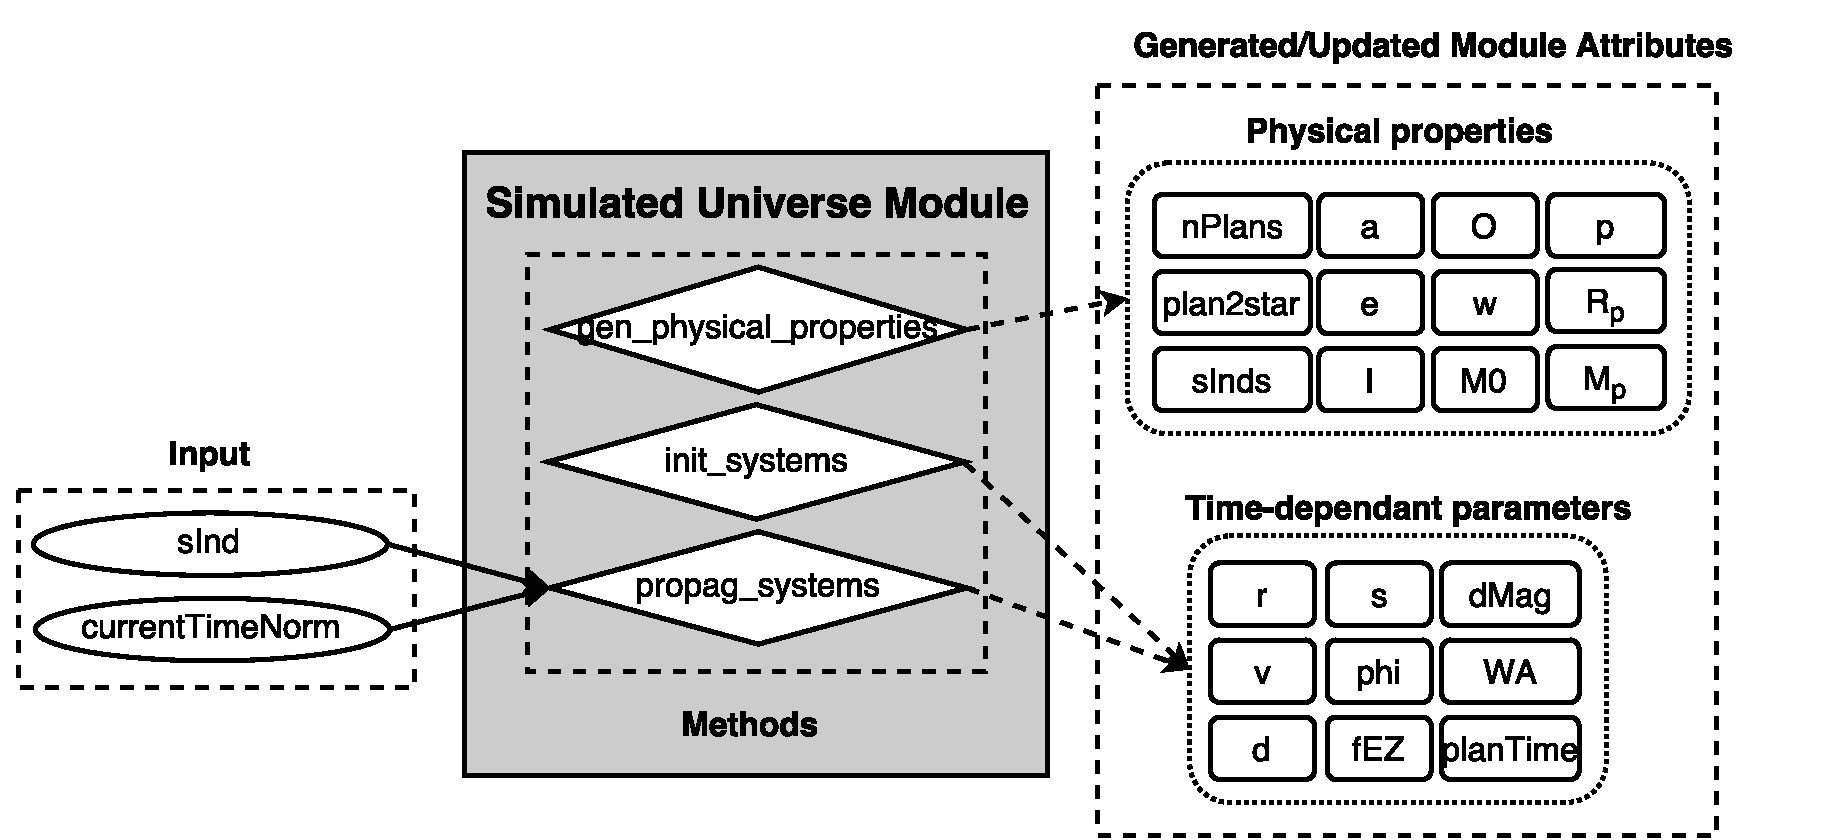
\includegraphics[width=\textwidth]{SimulatedUniverseTasks2}
        \end{tabular}
    \end{center}
    \caption{\label{fig:simulateduniversemodule} Depiction of Simulated Universe module methods including input and updated attributes (see \ref{sec:genphysicalpropertiestask}, \ref{sec:initsystemstask}, \ref{sec:propagsystemtask}, \ref{sec:dumpsystemstask}, \ref{sec:dumpsystemparamstask}, \ref{sec:reviseplanetslisttask}, and \ref{sec:revisestarslisttask}).}
\end{figure}

\subsubsection{Attributes}
\begin{itemize}
\item
\begin{description}
    \item[StarCatalog (StarCatalog module)]\hfill \\ StarCatalog class object (only retained if keepStarCatalog is True, see \ref{sec:starcatalog})
    \item[PlanetPopulation (PlanetPopulation module)] \hfill \\ PlanetPopulation class object (see \ref{sec:planetpopulation})
    \item[PlanetPhysicalModel (PlanetPhysicalModel module)] \hfill \\ PlanetPhysicalModel class object (see \ref{sec:planetphysicalmodel})
    \item[OpticalSystem (OpticalSystem module)] \hfill \\ OpticalSystem class object (see \ref{sec:opticalsystem})
    \item[ZodiacalLight (ZodiacalLight module)] \hfill \\ ZodiacalLight class object (see \ref{sec:zodiacallight})
    \item[BackgroundSources (BackgroundSources module)] \hfill \\ BackgroundSources class object (see \ref{sec:backgroundsources})
    \item[PostProcessing (PostProcessing module)] \hfill \\ PostProcessing class object (see \ref{sec:postprocessing})
    \item[Completeness (Completeness module)] \hfill \\ Completeness class object (see \ref{sec:completeness})
    \item[TargetList (TargetList module)] \hfill \\ TargetList class object (see \ref{sec:targetlist})
    \item[nPlans (integer)] \hfill \\ Total number of planets
    \item[plan2star (integer ndarray)] \hfill \\ Indices mapping planets to target stars in TargetList
    \item[sInds (integer ndarray)] \hfill \\ Unique indices of stars with planets in TargetList
    \item[a (astropy Quantity array)] \hfill \\ Planet semi-major axis in units of $ AU $
    \item[e (float ndarray)] \hfill \\ Planet eccentricity
    \item[I (astropy Quantity array)] \hfill \\ Planet inclination in units of $ deg $
    \item[O (astropy Quantity array)] \hfill \\ Planet right ascension of the ascending node in units of $ deg $
    \item[w (astropy Quantity array)] \hfill \\ Planet argument of perigee in units of $ deg $
    \item[Min (float)] \hfill \\ Constant initial mean anomaly for all planets (optional)
    \item[M0 (astropy Quantity array)] \hfill \\ Initial mean anomaly in units of $ deg $
    \item[p (float ndarray)] \hfill \\ Planet albedo
    \item[Rp (astropy Quantity array)] \hfill \\ Planet radius in units of $earthRad$
    \item[Mp (astropy Quantity array)] \hfill \\ Planet mass in units of $earthMass$
    \item[r (astropy Quantity n$\times$3 array)] \hfill \\ Planet position vector in units of $ AU $
    \item[v (astropy Quantity n$\times$3 array)] \hfill \\ Planet velocity vector in units of $ AU/day $
    \item[d (astropy Quantity array)] \hfill \\ Planet-star distances in units of $ AU $
    \item[s (astropy Quantity array)] \hfill \\ Planet-star apparent separations in units of $ AU $
    \item[phi (float ndarray)] \hfill \\ Planet phase function, given its phase angle
    \item[fEZ (astropy Quantity array)] \hfill \\ Surface brightness of exozodiacal light in units of $ 1/arcsec2 $, determined from \verb+ZodiacalLight.fEZ+ \S\ref{sec:fEZtask}
    \item[dMag (float ndarray)] \hfill \\ Differences in magnitude between planets and their host star
    \item[WA (astropy Quantity array)] \hfill \\ Working angles of the planets of interest in units of $arcsec$
\end{description}
\end{itemize}

\subsubsection{gen\_physical\_properties Method} \label{sec:genphysicalpropertiestask}
The \verb+gen_physical_properties+ method generates the planetary systems for the current simulated universe. This routine populates arrays of the orbital elements and physical characteristics of all planets, and generates indexes that map from planet to parent star. This method does not take any explicit inputs.  It uses the inherited TargetList and PlanetPopulation modules.

\subsubsection*{Generated Module Attributes}
\begin{itemize}
\item 
\begin{description}
    \item[nPlans (integer)] \hfill \\ Total number of planets
    \item[plan2star (integer ndarray)] \hfill \\ Indices mapping planets to target stars in TargetList
    \item[sInds (integer ndarray)] \hfill \\ Unique indices of stars with planets in TargetList
    \item[a (astropy Quantity array)] \hfill \\ Planet semi-major axis in units of $ AU $
    \item[e (float ndarray)] \hfill \\ Planet eccentricity
    \item[I (astropy Quantity array)] \hfill \\ Planet inclination in units of $ deg $
    \item[O (astropy Quantity array)] \hfill \\ Planet right ascension of the ascending node in units of $ deg $
    \item[w (astropy Quantity array)] \hfill \\ Planet argument of perigee in units of $ deg $
    \item[M0 (astropy Quantity array)] \hfill \\ Initial mean anomaly in units of $ deg $
    \item[p (float ndarray)] \hfill \\ Planet albedo
    \item[Mp (astropy Quantity array)] \hfill \\ Planet mass in units of $earthMass$
    \item[Rp (astropy Quantity array)] \hfill \\ Planet radius in units of $earthRad$
\end{description}
\end{itemize}

\subsection{gen\_M0 Method} \label{sec:genM0task}
The \verb+gen_M0+ method generates the constant or random initial mean anomaly for each simulated planet inside of \verb+gen_physical_properties+. This method does not take any explicit inputs.

\subsubsection*{Output}
\begin{itemize}
    \item 
    \begin{description}
        \item[M0 (astropy Quantity array)] \hfill \\
        Initial mean anomalies in units of $deg$
    \end{description}
\end{itemize}

\subsubsection{init\_systems Method} \label{sec:initsystemstask}
The \verb+init_systems+ method finds initial time-dependant parameters. It assigns each planet an initial position, velocity, planet-star distance, apparent separation, phase function, delta magnitude, working angle, surface brightness of exo-zodiacal light, and initializes the planet current times to zero. This method does not take any explicit inputs.  It uses the following attributes assigned before calling this method:
\begin{itemize}
    \item \verb+SimulatedUniverse.a+
    \item \verb+SimulatedUniverse.e+
    \item \verb+SimulatedUniverse.I+
    \item \verb+SimulatedUniverse.O+
    \item \verb+SimulatedUniverse.w+
    \item \verb+SimulatedUniverse.M0+
    \item \verb+SimulatedUniverse.p+
    \item \verb+SimulatedUniverse.Mp+
    \item \verb+SimulatedUniverse.Rp+
    \item \verb+TargetList.MV+
    \item \verb+TargetList.dist+
\end{itemize}

\subsubsection*{Generated Module Attributes}
\begin{itemize}
\item 
\begin{description}
    \item[r (astropy Quantity n$\times$3 array)] \hfill \\ Planet position vector in units of $ AU $
    \item[v (astropy Quantity n$\times$3 array)] \hfill \\ Planet velocity vector in units of $ AU/day $
    \item[d (astropy Quantity array)] \hfill \\ Planet-star distances in units of $ AU $
    \item[s (astropy Quantity array)] \hfill \\ Planet-star apparent separations in units of $ AU $
    \item[phi (float ndarray)] \hfill \\ Planet phase function given its phase angle, determined from \verb+PlanetPhysicalModel.calc_Phi+ \S\ref{sec:planetphysicalmodel}
    \item[fEZ (astropy Quantity array)] \hfill \\ Surface brightness of exozodiacal light in units of $ 1/arcsec2 $, determined from \verb+ZodiacalLight.fEZ+ \S\ref{sec:fEZtask}
    \item[dMag (float ndarray)] \hfill \\ Differences in magnitude between planets and their host star
    \item[WA (astropy Quantity array)] \hfill \\ Working angles of the planets of interest in units of $arcsec$
\end{description}
\end{itemize}

\subsubsection{propag\_system Method} \label{sec:propagsystemtask}
The \verb+propag_system+ method propagates planet time-dependant parameters: position, velocity, planet-star distance, apparent separation, and surface brightness of exo-zodiacal light.

\subsubsection*{Input}
\begin{itemize}
\item 
\begin{description}
    \item[sInd (integer)] \hfill \\ Index of the target system of interest
    \item[dt (astropy Quantity)] \hfill \\ Time increment in units of $day$, for planet position propagation
\end{description}
\end{itemize}

\subsubsection*{Updated Module Attributes}
\begin{itemize}
\item 
\begin{description}
    \item[r (astropy Quantity n$\times$3 array)] \hfill \\ Planet position vector in units of $ AU $
    \item[v (astropy Quantity n$\times$3 array)] \hfill \\ Planet velocity vector in units of $ AU/day $
    \item[d (astropy Quantity array)] \hfill \\ Planet-star distances in units of $ AU $
    \item[s (astropy Quantity array)] \hfill \\ Planet-star apparent separations in units of $ AU $
    \item[phi (float ndarray)] \hfill \\ Planet phase function given its phase angle, determined from \verb+PlanetPhysicalModel.calc_Phi+ \S\ref{sec:planetphysicalmodel}
    \item[fEZ (astropy Quantity array)] \hfill \\ Surface brightness of exozodiacal light in units of $ 1/arcsec2 $, determined from \verb+ZodiacalLight.fEZ+ \S\ref{sec:fEZtask}
    \item[dMag (float ndarray)] \hfill \\ Differences in magnitude between planets and their host star
    \item[WA (astropy Quantity array)] \hfill \\ Working angles of the planets of interest in units of $arcsec$
\end{description}
\end{itemize}

\subsubsection{dump\_systems Method} \label{sec:dumpsystemstask}
The \verb+dump_systems+ method creates a dictionary of planetary properties for archiving use.

\subsubsection*{Output}
\begin{itemize}
\item 
\begin{description}
    \item[systems (dict)] \hfill \\ Dictionary of planetary properties
\end{description}
\end{itemize}

\subsubsection{dump\_system\_params Method} \label{sec:dumpsystemparamstask}
The \verb+dump_system_params+ method creates a dictionary of time-dependant planet properties for a specific target.

\subsubsection*{Input}
\begin{itemize}
\item 
\begin{description}
    \item[sInd (integer)] \hfill \\ Index of the target system of interest
\end{description}
\end{itemize}

\subsubsection*{Output}
\begin{itemize}
\item 
\begin{description}
    \item[systems (dict)] \hfill \\ Dictionary of time-dependant planet properties
\end{description}
\end{itemize}

\subsubsection{revise\_planets\_list Method} \label{sec:reviseplanetslisttask}
The \verb+revise_planets_list+ method replaces Simulated Universe planet attributes with filtered values, and updates the number of planets.

\subsubsection*{Input}
\begin{itemize}
\item 
\begin{description}
    \item[pInds (integer ndarray)] \hfill \\  Planet indices to keep
\end{description}
\end{itemize}

\subsubsection{revise\_stars\_list Method} \label{sec:revisestarslisttask}
The \verb+revise_stars_list+ method revises the TargetList with filtered values, and updates the planets list accordingly.

\subsubsection*{Input}
\begin{itemize}
\item 
\begin{description}
    \item[sInds (integer ndarray)] \hfill \\  Star indices to keep
\end{description}
\end{itemize}


% OBSERVATORY

\subsection{Observatory}
The Observatory module contains all of the information specific to the space-based observatory not included in the Optical System module. The module has four main methods: \verb+orbit+, \verb+solarSystem_body_position+, \verb+keepout+, and \verb+distForces+, which are implemented as functions within the module. 

The observatory orbit plays a key role in determining which of the target stars may be observed for planet finding at a specific time during the mission lifetime. The Observatory module's \verb+orbit+ method takes the current mission time as input and outputs the observatory's position vector. The position vector is standardized throughout the modules to be referenced to a heliocentric equatorial frame at the J2000 epoch. The observatory's position vector is used in the \verb+keepout+ method to determine which of the stars are observable at the current mission time.

The position vectors of bright objects such as the sun, the moon, and the solar system planets, are calculated by the \verb+solarSystem_body_position+ method. 

The \verb+keepout+ method determines which target stars are observable at a specific time during the mission simulation and which are unobservable due to bright objects within the field of view. The keepout volume is determined by the specific design of the observatory and, in certain cases, by the starlight suppression system.  The \verb+keepout+ method takes the Target List module and current mission time as inputs and outputs a list of the target stars which are observable at the current time. It constructs position vectors of the target stars and bright objects which may interfere with observations with respect to the observatory. These position vectors are used to determine if bright objects are in the field of view for each of the potential stars under exoplanet finding observation.  If there are no bright objects obstructing the view of the target star, it becomes a candidate for observation in the Survey Simulation module.  The solar keepout is typically encoded as allowable angle ranges for the spacecraft-star unit vector as measured from the spacecraft-sun vector.

Finally, the \verb+distForces+ method determines the lateral and axial disturbance forces that apply on an external occulter (i.e., starshade).

In addition to these methods, the observatory definition can also encode finite resources used by the observatory throughout the mission.  The most important of these is the fuel used for stationkeeping and repointing, especially in the case of occulters which must move significant distances between observations.  Other considerations could include the use of other volatiles such as cryogens for cooled instruments, which tend to deplete solely as a function of mission time.  This module also allows for detailed investigations of the effects of orbital design on the science yield, e.g., comparing the original baseline geosynchronous 28.5\textdegree{} inclined orbit for WFIRST with an L2 halo orbit, which is the new mission baseline. 

The input and output of the Observatory module methods are depicted in \reffig{fig:observatorymodule}.

\begin{figure}[ht]
    \begin{center}
        \begin{tabular}{c}
             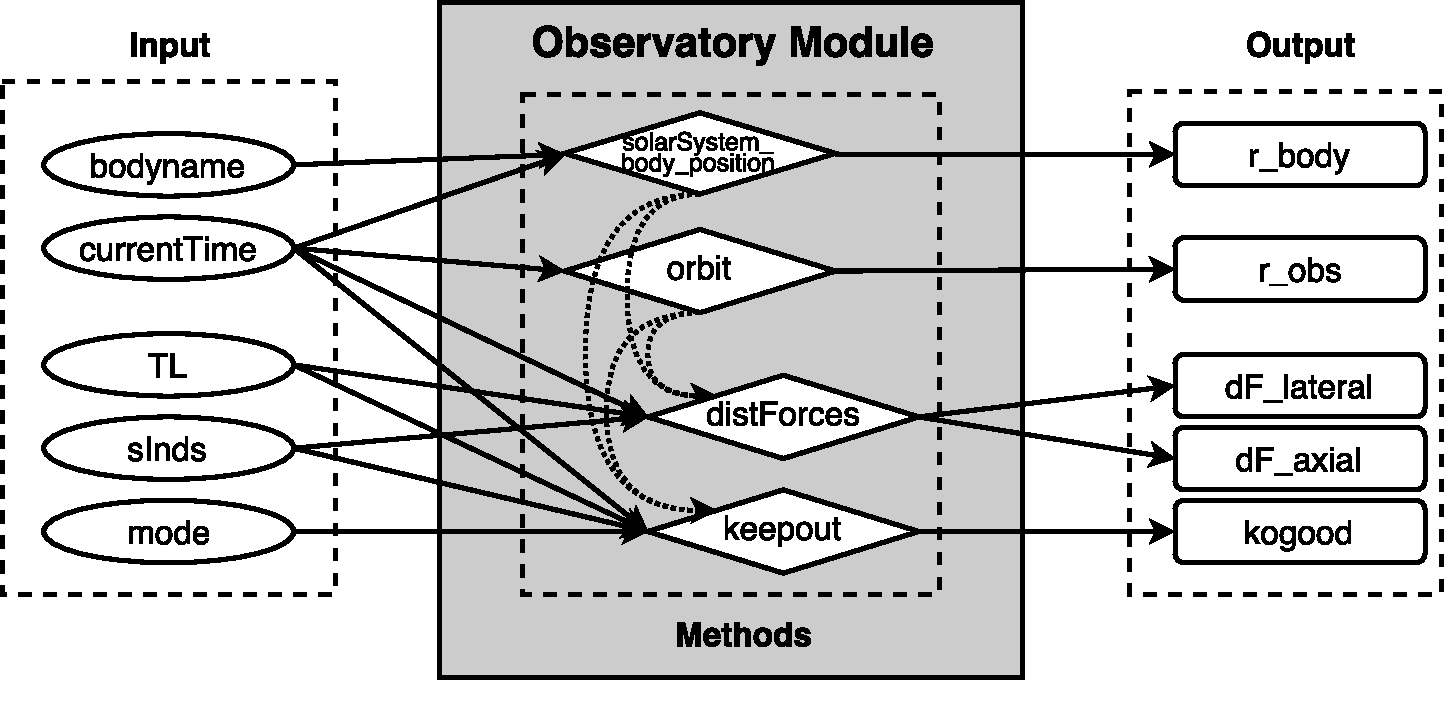
\includegraphics[width=0.9\textwidth]{observatory4}
        \end{tabular}
    \end{center}
    \caption{\label{fig:observatorymodule} Depiction of Observatory module methods including input and output (see \S\ref{sec:orbittask}, \S\ref{sec:ssbPosTask}, \S\ref{sec:keepouttask}, and \S\ref{sec:distforcestask}).}
\end{figure}

\label{sec:observatory}
\subsubsection{Observatory Object Attribute Initialization}

\subsubsection*{Input}
\begin{itemize}
\item
\begin{description}
    \item[koAngleMin (float)] \hfill \\ Telescope minimum keepout angle in units of $deg$. Default value is 45.
    \item[koAngleMinMoon (float)] \hfill \\ Telescope minimum keepout angle in units of $deg$, for the Moon only. Defaults to koAngleMin.
    \item[koAngleMinEarth (float)] \hfill \\ Telescope minimum keepout angle in units of $deg$, for the Earth only. Defaults to koAngleMin.
    \item[koAngleMax (float)] \hfill \\ Telescope maximum keepout angle (for occulter) in units of $deg$. Default value is 90.
    \item[koAngleSmall (float)] \hfill \\ Telescope keepout angle for smaller (angular size) bodies in units of $deg$. Default value is 1.
    \item[checkKeepoutEnd (boolean)] \hfill \\ Boolean signifying if the keepout method must be called at the end of each observation.
    \item[settlingTime (float)] \hfill \\ Amount of time needed for observatory to settle after a repointing in units of $ day $. Default value is 1.
    \item[thrust (float)] \hfill \\ Occulter slew thrust in units of $ mN $. Default value is 450.
    \item[slewIsp (float)] \hfill \\ Occulter slew specific impulse in units of $ s $. Default value is 4160.
    \item[scMass (float)] \hfill \\ Occulter (maneuvering spacecraft) initial wet mass in units of $ kg $. Default value is 6000.
    \item[dryMass (float)] \hfill \\ Occulter (maneuvering spacecraft) dry mass in units of $ kg $. Default value is 3400.
    \item[coMass (float)] \hfill \\ Telescope (or non-maneuvering spacecraft) mass in units of $ kg $. Default value is 5800.
    \item[occulterSep (float)] \hfill \\ Occulter-telescope distance in units of $ km $. Default value is 55000.
    \item[skIsp (float)] \hfill \\ Specific impulse for station keeping in units of $ s $. Default value is 220.
    \item[defburnPortion (float)] \hfill \\ Default burn portion for slewing. Default value is 0.05
    \item[checkKeepoutEnd (boolean)] \hfill \\ Boolean signifying if the keepout method must be called at the end of each observation. Default value is True.
    \item[forceStaticEphem (boolean)] \hfill \\ Boolean, forcing use of static solar system ephemeris if set to True, even if jplephem module is present (see \ref{sec:ssbPosTask}).  Default value is False.
    \item[spkpath (string)] \hfill\\ String with full path to SPK kernel file (only used if using jplephem for solar system body propagation - see \ref{sec:ssbPosTask}).
\end{description}
\end{itemize}

\subsubsection*{Attributes}
\begin{itemize}
\item
\begin{description}
    \item[koAngleMin (astropy Quantity)] \hfill \\ Telescope minimum keepout angle in units of $deg$
    \item[koAngleMinMoon (astropy Quantity)] \hfill \\ Telescope minimum keepout angle in units of $deg$, for the Moon only
    \item[koAngleMinEarth (astropy Quantity)] \hfill \\ Telescope minimum keepout angle in units of $deg$, for the Earth only
    \item[koAngleMax (astropy Quantity)] \hfill \\ Telescope maximum keepout angle (for occulter) in units of $deg$
    \item[koAngleSmall (astropy Quantity)] \hfill \\ Telescope keepout angle for smaller (angular size) bodies in units of $deg$
    \item[settlingTime (astropy Quantity)] \hfill \\ Amount of time needed for observatory to settle after a repointing in units of $ day $
    \item[thrust (astropy Quantity)] \hfill \\ Occulter slew thrust in units of $ mN $
    \item[slewIsp (astropy Quantity)] \hfill \\ Occulter slew specific impulse in units of $ s $
    \item[scMass (astropy Quantity)] \hfill \\ Occulter (maneuvering spacecraft) initial wet mass in units of $ kg $
    \item[dryMass (astropy Quantity)] \hfill \\ Occulter (maneuvering spacecraft) dry mass in units of $ kg $
    \item[coMass (astropy Quantity)] \hfill \\ Telescope (or non-maneuvering spacecraft) mass in units of $ kg $
    \item[occulterSep (astropy Quantity)] \hfill \\ Occulter-telescope distance in units of $ km $
    \item[skIsp (astropy Quantity)] \hfill \\ Specific impulse for station keeping in units of $ s $
    \item[defburnPortion (float)] \hfill \\ Default burn portion for slewing
    \item[flowRate (astropy Quantity)] \hfill \\ Slew flow rate derived from thrust and slewIsp in units of $ kg/day $
    \item[checkKeepoutEnd (boolean)] \hfill \\ Boolean signifying if the keepout method must be called at the end of each observation
    \item[forceStaticEphem (boolean)] \hfill \\ Boolean, forcing use of static solar system ephemeris if set to True.
\end{description}
\end{itemize}

\subsubsection{orbit Method} \label{sec:orbittask}
The \verb+orbit+ method finds the heliocentric equatorial position vector of the observatory spacecraft.

\subsubsection*{Input}
\begin{itemize}
\item
\begin{description}
    \item[currentTime (astropy \href{http://astropy.readthedocs.org/en/latest/time/index.html}{Time} array)] \hfill \\ Current absolute mission time in MJD
\end{description}
\end{itemize}

\subsubsection*{Output}
\begin{itemize}
\item
\begin{description}
    \item[r\_sc (astropy Quantity n$\times$3 array)] \hfill \\ Observatory orbit position in HE reference frame at current mission time in units of $ km $
\end{description}
\end{itemize}

\subsubsection{solarSystem\_body\_position Method}\label{sec:ssbPosTask}
The \verb+solarSystem_body_position+ returns the position of any solar system body (Earth, Sun, Moon, etc.) at a given time in the common Heliocentric Equatorial frame.  The observatory prototype will attempt to load the jplephem module, and use a local SPK file for all propagations if available.  The SPK file is not packaged with the software but may be downloaded from JPL's website at: \url{http://naif.jpl.nasa.gov/pub/naif/generic_kernels/spk/planets/a_old_versions/}.  The location of the spk file is assumed to be in the Observatory directory but can be set by the \verb+spkpath+ input.  

If jplephem is not present, the Observatory prototype will load static ephemeris derived from Vallado (2004) and use those for propagation.  This behavior can be forced even when jplephem is available by setting the \verb+forceStaticEphem+ input to True.

\subsubsection*{Input}
\begin{itemize}
\item
\begin{description}
    \item[currentTime (astropy \href{http://astropy.readthedocs.org/en/latest/time/index.html}{Time})] \hfill \\ Current absolute mission time in MJD
    \item[bodyname (string)] \hfill \\ Solar system object name, capitalized by convention
\end{description}
\end{itemize}

\subsubsection*{Output}
\begin{itemize}
\item
\begin{description}
    \item[r\_body (astropy Quantity n$\times$3 array)] \hfill \\ Heliocentric equatorial position vector in units of $ km $
\end{description}
\end{itemize}


\subsubsection{keepout Method} \label{sec:keepouttask} 
The \verb+keepout+ method determines which stars in the target list are observable at the given input time.

\subsubsection*{Input}
\begin{itemize}
\item
\begin{description}
    \item[TL (TargetList module)] \hfill \\ TargetList class object, see \S\ref{sec:targetlist} for definition of available attributes
    \item[sInds (integer ndarray)] \hfill \\ Integer indices of the stars of interest
    \item[currentTime (astropy \href{http://astropy.readthedocs.org/en/latest/time/index.html}{Time} array)] \hfill \\ Current absolute mission time in MJD
    \item[mode (dict)] \hfill \\ Selected observing mode (from OpticalSystem)
\end{description}
\end{itemize}

\subsubsection*{Output}
\begin{itemize}
\item 
\begin{description}
    \item[kogood (boolean ndarray)] \hfill \\ True is a target unobstructed and observable, and False is a target unobservable due to obstructions in the keepout zone.
\end{description}
\end{itemize}

\subsubsection{distForces Method} \label{sec:distforcestask} 
The \verb+distForces+ method finds lateral and axial disturbance forces on an occulter .

\subsubsection*{Input}
\begin{itemize}
\item
\begin{description}
    \item[TL (TargetList module)] \hfill \\ TargetList class object, see \S\ref{sec:targetlist} for definition of available attributes
    \item[sInd (integer)] \hfill \\ Integer index of the star of interest
    \item[currentTime (astropy \href{http://astropy.readthedocs.org/en/latest/time/index.html}{Time} array)] \hfill \\ Current absolute mission time in MJD
\end{description}
\end{itemize}

\subsubsection*{Output}
\begin{itemize}
\item 
\begin{description}
    \item[dF\_lateral (astropy Quantity)] \hfill \\ Lateral disturbance force in units of $N$
    \item[dF\_axial (astropy Quantity)] \hfill \\ Axial disturbance force in units of $N$
\end{description}
\end{itemize}


% TIME KEEPING 

\subsection{Time Keeping} \label{sec:timekeeping}
The Time Keeping module is responsible for keeping track of the current mission time.  It encodes only the mission start time, the mission duration, and the current time within a simulation.  All functions in all modules requiring knowledge of the current time call functions or access parameters implemented within the Time module.  Internal encoding of time is implemented as the time from mission start (measured in units of $ day $).  The Time Keeping module also provides functionality for converting between this time measure and standard measures such as Julian Day Number and UTC time.
 
The input, output and updated attributes of the Time Keeping methods are depicted in \reffig{fig:timekeepingmodule}. The Time Keeping module contains two methods:

\begin{itemize}[leftmargin=1.5in,font={\ttfamily}]
    \item[\texttt allocate\_time] Allocates a temporal block of width $dt$, advancing the observation window if needed, and updates the mission time during a survey simulation (see \S\ref{sec:allocatetimetask})
    \item[\texttt next\_observing\_block] Defines the next observing block, start and end times (see \S\ref{sec:nextOBtask})
    \item[\texttt mission\_is\_over] Checks if the time allocated for the mission is used up (see \S\ref{sec:missionisovertask})
\end{itemize}

\begin{figure}[ht]
    \begin{center}
        \begin{tabular}{c}
             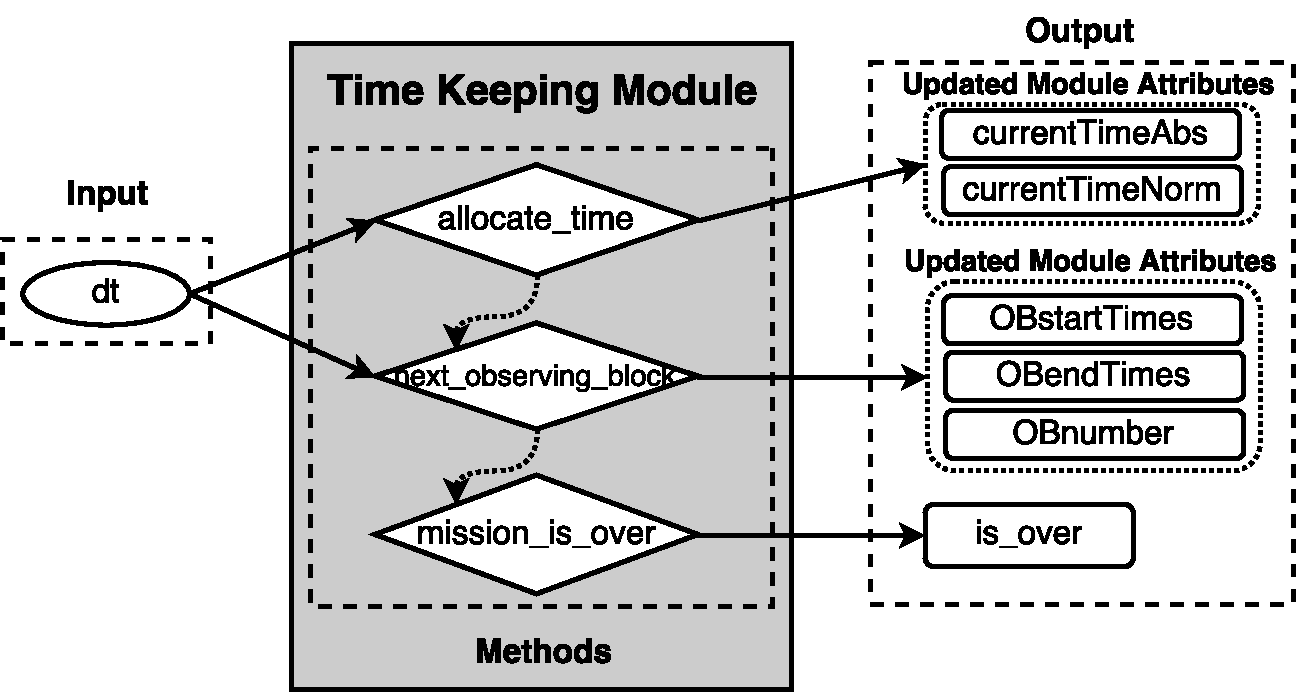
\includegraphics[width=\textwidth]{TimeKeepingTasks3}
        \end{tabular}
    \end{center}
    \caption{\label{fig:timekeepingmodule} Depiction of Time Keeping module method including input, output, and updated attributes (see \S\ref{sec:allocatetimetask}, \S\ref{sec:nextOBtask}, and \S\ref{sec:missionisovertask}).}
\end{figure}

\subsubsection{Time Keeping Object Attribute Initialization}

\subsubsection*{Input}
\begin{itemize}
\item
\begin{description}
    \item[missionStart (float)] \hfill \\ Mission start time in $ MJD $. Default value is 60634.
    \item[missionLife (float)] \hfill \\ Total length of mission in units of $ year $. Default value is 6.
    \item[extendedLife (float)] \hfill \\ Extended mission time in units of $ year $. Default value is 0.  Extended life typically differs from the primary mission in some way---most typically only revisits are allowed.
    \item[missionPortion (float)] \hfill \\ Portion of mission time devoted to planet-finding. Default value is 1/6.
    \item[OBduration (float)] \hfill \\ Default allocated duration of observing blocks, in units of $day$. If no OBduration was specified, a new observing block is created for each new observation in the SurveySimulation module.
    \item[waitTime (float)] \hfill \\ Default allocated duration to wait in units of $day$, when the Survey Simulation does not find any observable target. Default value is 1.
    \item[waitMultiple (float)] \hfill \\ Multiplier applied to the wait time in case of repeated empty lists of observable targets, which makes the wait time grow exponentially. Default value is 2.
\end{description}
\end{itemize}

\subsubsection*{Attributes}
\begin{itemize}
\item
\begin{description}
    \item[missionStart (astropy \href{http://astropy.readthedocs.org/en/latest/time/index.html}{Time})] \hfill \\
        Mission start time in $ MJD $
    \item[missionLife (astropy Quantity)] \hfill \\ Mission lifetime in units of $ year $
    \item[extendedLife (astropy Quantity)] \hfill \\ Extended mission time in units of $ year $
    \item[missionPortion (float)] \hfill \\ Portion of mission time devoted to planet-finding
    \item[missionFinishNorm] \hfill \\ Mission finish time in units of $ day $
    \item[missionFinishAbs (astropy \href{http://astropy.readthedocs.org/en/latest/time/index.html}{Time})] \hfill \\ Mission completion date in $ MJD $
    \item[currentTimeNorm (astropy Quantity)] \hfill \\ Current mission time normalized so that start date is 0, in units of $ day $
    \item[currentTimeAbs (astropy \href{http://astropy.readthedocs.org/en/latest/time/index.html}{Time})] \hfill \\ Current absolute mission time in $ MJD $
    \item[OBnumber (integer)] \hfill \\ Index/number associated with the current observing block (OB). Each observing block has a duration, a start time, an end time, and can host one or multiple observations.
    \item[OBduration (astropy Quantity)] \hfill \\ Default allocated duration of observing blocks, in units of $day$. If no OBduration was specified, a new observing block is created for each new observation in the SurveySimulation module. 
    \item[OBstartTimes (astropy Quantity array)] \hfill \\ Array containing the normalized start times of each observing block throughout the mission, in units of $day$
    \item[OBendTimes (astropy Quantity array)] \hfill \\ Array containing the normalized end times of each observing block throughout the mission, in units of $day$
    \item[obsStart (astropy Quantity)] \hfill \\ Normalized start time of the observation currently executed by the Survey Simulation, in units of $day$
    \item[obsEnd (astropy Quantity)] \hfill \\ Normalized end time of the observation currently executed by the Survey Simulation, in units of $day$
    \item[waitTime (astropy Quantity)] \hfill \\ Default allocated duration to wait in units of $day$, when the Survey Simulation does not find any observable target
    \item[waitMultiple (float)] \hfill \\ Multiplier applied to the wait time in case of repeated empty lists of observable targets, which makes the wait time grow exponentially. As soon as an observable target is found, the wait time is reinitialized to the default waitTime value.


\end{description}
\end{itemize}

\subsubsection{allocate\_time Method} \label{sec:allocatetimetask}

\subsubsection*{Input}
\begin{itemize}
\item 
\begin{description}
    \item[dt (astropy Quantity)] \hfill \\ Amount of time requested in units of day
\end{description}
\end{itemize}

\subsubsection*{Updated Module Attributes}
\begin{itemize}
\item 
\begin{description}
    \item[currentTimeNorm (astropy Quantity)] \hfill \\ Current mission time normalized so that start date is 0, in units of $ day $
    \item[currentTimeAbs (astropy \href{http://astropy.readthedocs.org/en/latest/time/index.html}{Time})] \hfill \\ Current absolute mission time in $ MJD $
\end{description}
\end{itemize}

\subsubsection{next\_observing\_block Method} \label{sec:nextOBtask}

\subsubsection*{Input}
\begin{itemize}
\item 
\begin{description}
    \item[dt (astropy Quantity)] \hfill \\ Amount of time requested in units of day
\end{description}
\end{itemize}

\subsubsection*{Updated Module Attributes}
\begin{itemize}
\item 
\begin{description}
    \item[OBstartTimes (astropy Quantity array)] \hfill \\ Array containing the normalized start times of each observing block throughout the mission, in units of $day$
    \item[OBendTimes (astropy Quantity array)] \hfill \\ Array containing the normalized end times of each observing block throughout the mission, in units of $day$
    \item[OBnumber (integer)] \hfill \\ Index/number associated with the current observing block (OB). Each observing block has a duration, a start time, an end time, and can host one or multiple observations.
\end{description}
\end{itemize}

\subsubsection{mission\_is\_over Method} \label{sec:missionisovertask}
The \verb+mission_is_over+ method does not take any explicit inputs.  It uses the updated module attribute \verb+currentTimeNorm+.

\subsubsection*{Output}
\begin{itemize}
\item 
\begin{description}
    \item[is\_over (boolean)] \hfill \\ True if the mission time is used up, else False
\end{description}
\end{itemize}


% SURVEY SIMULATION

\subsection{Survey Simulation} \label{sec:surveysim}
This is the module that performs a specific simulation based on all of the input parameters and models. This module returns the mission timeline - an ordered list of simulated observations of various targets on the target list along with their outcomes.  The output also includes an encoding of the final state of the simulated universe (so that a subsequent simulation can start from where a previous simulation left off) and the final state of the observatory definition (so that post-simulation analysis can determine the percentage of volatiles expended, and other engineering metrics).

The input, output and updated attributes of the Survey Simulation methods are depicted in \reffig{fig:surveysimulationmodule}. The Survey Simulation module contains the following methods:
\begin{itemize}[leftmargin=2.5in,font={\ttfamily}]
    \item[\texttt run\_sim] Performs the survey simulation (see \S\ref{sec:runsimtask})
    \item[\texttt next\_target] Finds index of next target star and calculates its integration time (see \S\ref{sec:nexttargettask})
    \item[\texttt observation\_detection] Determines detection status for a given integration time  (see \S\ref{sec:observationdetectiontask})
    \item[\texttt observation\_characterization] Determines characterization time and status (see \S\ref{sec:observationcharacterizationtask})
    \item[\texttt calc\_signal\_noise] Calculates the signal and noise fluxes for a given time interval (see \S\ref{sec:calcsignalnoisetask}) - called by \verb+observation_detection+ and \verb+observation_characterization+
    \item[\texttt update\_occulter\_mass] Updates the occulter wet mass in the Observatory module, and stores all the occulter related values in the DRM array (see \S\ref{sec:updateoccultermasstask})
\end{itemize}

\begin{figure}[ht]
    \begin{center}
        \begin{tabular}{c}
            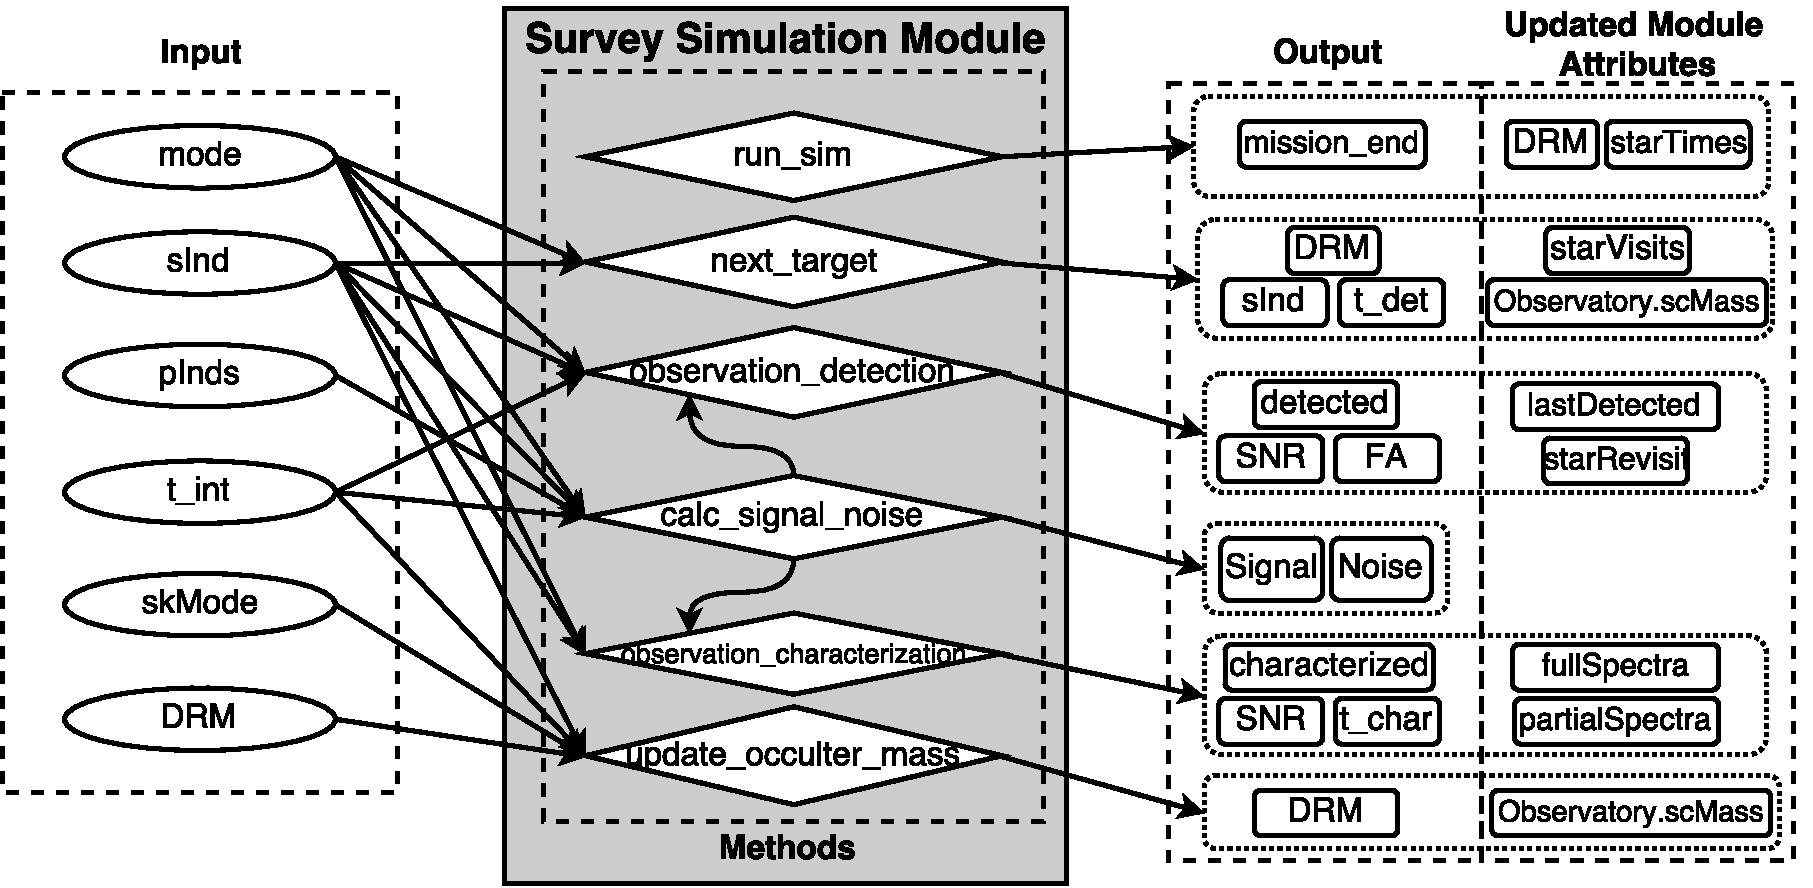
\includegraphics[width=\textwidth]{SurveySimulation}
        \end{tabular}
    \end{center}
    \caption{\label{fig:surveysimulationmodule} Depiction of Survey Simulation module method including input, output, and updated attributes (see \S\ref{sec:runsimtask}, \S\ref{sec:nexttargettask}, \S\ref{sec:observationdetectiontask}, \S\ref{sec:observationcharacterizationtask}, \S\ref{sec:calcsignalnoisetask} and \S\ref{sec:updateoccultermasstask}).}
\end{figure}

\subsubsection{Survey Simulation Object Attribute Initialization}

\subsubsection*{Input}
\begin{itemize}
\item 
\begin{description}
    \item[scriptfile (string)] \hfill \\ JSON script file.  If not set, assumes that dictionary has been passed through specs.
    \item[nt\_flux (integer)] \hfill \\ Observation time sampling, to determine the integration time interval. Default value is 1.
    \item[nVisitsMax (integer)] \hfill \\ Maximum number of observations (in detection mode) per star. Default value is 5.
    \item[charMargin (float)] \hfill \\ Integration time margin for characterization. Default value is 15.
    \item[seed (integer)] \hfill \\ Random seed used to make all random number generation reproducible.
    \item[WAint (float)] \hfill \\ Working angle used for integration time calculation in units of $arcsec$.
    \item[dMagint (float)] \hfill \\ Delta magnitude used for integration time calculation.
\end{description}
\end{itemize}

\subsubsection*{Attributes}
\begin{itemize}
\item
\begin{description}
    \item[StarCatalog (StarCatalog module)]\hfill \\ StarCatalog class object (only retained if keepStarCatalog is True, see \ref{sec:starcatalog})
    \item[PlanetPopulation (PlanetPopulation module)] \hfill \\ PlanetPopulation class object (see \ref{sec:planetpopulation})
    \item[PlanetPhysicalModel (PlanetPhysicalModel module)] \hfill \\ PlanetPhysicalModel class object (see \ref{sec:planetphysicalmodel})
    \item[OpticalSystem (OpticalSystem module)] \hfill \\ OpticalSystem class object (see \ref{sec:opticalsystem})
    \item[ZodiacalLight (ZodiacalLight module)] \hfill \\ ZodiacalLight class object (see \ref{sec:zodiacallight})
    \item[BackgroundSources (BackgroundSources module)] \hfill \\ BackgroundSources class object (see \ref{sec:backgroundsources})
    \item[PostProcessing (PostProcessing module)] \hfill \\ PostProcessing class object (see \ref{sec:postprocessing})
    \item[Completeness (Completeness module)] \hfill \\ Completeness class object (see \ref{sec:completeness})
    \item[TargetList (TargetList module)] \hfill \\ TargetList class object (see \ref{sec:targetlist})
    \item[SimulatedUniverse (SimulatedUniverse module)] \hfill \\ SimulatedUniverse class object (see \ref{sec:simulateduniverse})
    \item[Observatory (Observatory module)] \hfill \\ Observatory class object (see \ref{sec:observatory})
    \item[TimeKeeping (TimeKeeping module)] \hfill \\ TimeKeeping class object (see \ref{sec:timekeeping})
    \item[fullSpectra (boolean ndarray)] \hfill \\ Indicates if planet spectra have been captured
    \item[partialSpectra (boolean ndarray)] \hfill \\ Indicates if planet partial spectra have been captured
    \item[propagTimes (astropy Quantity array)] \hfill \\ Contains the last time the stellar system was propagated in units of $day$
    \item[lastObsTimes (astropy Quantity array)] \hfill \\ Contains the last observation start time for future completeness update in units of $day$
    \item[starVisits (integer ndarray)] \hfill \\ Contains the number of times each target was visited
    \item[starRevisit (float n$\times$2 ndarray)] \hfill \\ Contains indices of targets to revisit and revisit times of these targets in units of $day$
    \item[starExtended (integer ndarray)] \hfill \\ Contains indices of targets with detected planets, updated throughout the mission
    \item[lastDetected (float n$\times$4 ndarray)] \hfill \\ For each target, contains 4 lists with planets' detected status, exozodi brightness (in units of $1/arcsec^2$), delta magnitude, and working angles (in units of $arcsec$)
    \item[DRM (list of dicts)] \hfill \\ Design Reference Mission, contains the results of a survey simulation
    \item[nt\_flux (integer)] \hfill \\ Observation time sampling, to determine the integration time interval
    \item[nVisitsMax (integer)] \hfill \\ Maximum number of observations (in detection mode) per star
    \item[charMargin (float)] \hfill \\ Integration time margin for characterization
    \item[seed (integer)] \hfill \\ Random seed used to make all random number generation reproducible
    \item[WAint (astropy Quantity array)] \hfill \\ Working angle used for integration time calculation in units of $arcsec$
    \item[dMagint (float ndarray)] \hfill \\ Delta magnitude used for integration time calculation
\end{description}
\end{itemize}

\subsubsection{run\_sim Method} \label{sec:runsimtask}
The \verb+run_sim+ method uses the inherited modules to generate a survey simulation, without any explicit inputs and outputs. It updates module attributes and populates the results in \verb+SurveySimulation.DRM+.

\subsubsection*{Updated Module Attributes}
\begin{itemize}
\item 
\begin{description}
    \item[SurveySimulation.DRM] \hfill \\ Python list where each entry contains a dictionary of survey simulation results for each observation.  The dictionary may include the following \verb+key:value+ pairs (from the prototype):
    \begin{description}
        \item[star\_ind (integer)] \hfill \\ Index of the observed target star
        \item[star\_name (string)] \hfill \\ Name of the observed target star
        \item[arrival\_time (float)] \hfill \\ Elapsed time since mission start when observation begins in units of $day$
        \item[OB\_nb (integer)] \hfill \\ Number/index of the observing block
        \item[plan\_inds (integer ndarray)] \hfill \\ Indices of planets orbiting the observed target star
        \item[det\_mode (dict)] \hfill \\ Observing mode selected for detection
        \item[det\_time (astropy Quantity)] \hfill \\ Integration time for detection in units of $ day $
        \item[det\_status (integer ndarray)] \hfill \\ List of detection status for each planet orbiting the observed target star, where 1 is detection, 0 missed detection, -1 below IWA, and -2 beyond OWA
        \item[det\_SNR (float ndarray)] \hfill \\ List of detection SNR values for each planet orbiting the observed target star. Non-observable planets have their SNR set to 0.
        \item[det\_fZ] (astropy Quantity)] \hfill \\ Zodiacal surface brightnesses at detection in units of $1/arcsec^2$
        \item[det\_params (dict)] \hfill \\ Dictionary of system params at detection for each planet orbiting the observed target star, including d ($AU$), phi, fEZ ($1/arcsec2$), dMag, and WA ($arcsec$)
        \item[char\_mode (dict)] \hfill \\ Observing mode selected for characterization
        \item[char\_time (astropy Quantity)] \hfill \\ Integration time for characterization in units of $ day $
        \item[char\_status (integer ndarray)] \hfill \\ List of characterization status for each planet orbiting the observed target star, where 1 is full spectrum, -1 partial spectrum, and 0 not characterized
        \item[char\_SNR (float ndarray)] \hfill \\ List of characterization SNR values for each planet orbiting the observed target star. Non-observable planets have their SNR set to 0.
        \item[char\_fZ] (astropy Quantity)] \hfill \\ Zodiacal surface brightnesses at characterization in units of $1/arcsec^2$
        \item[char\_params (dict)] \hfill \\ Dictionary of system params at characterization for each planet orbiting the observed target star, including d ($AU$), phi, fEZ ($1/arcsec2$), dMag, and WA ($arcsec$)
        \item[FA\_det\_status (integer)] \hfill \\ Detection status for a false alarm signal (1 is a false alarm, 0 is not)
        \item[FA\_char\_status (integer ndarray)] \hfill \\ (if false alarm) Characterization status for a false alarm signal, where 1 is full spectrum, -1 partial spectrum, and 0 not characterized
        \item[FA\_char\_SNR (float ndarray)] \hfill \\ (if false alarm) Characterization SNR value for a false alarm signal
        \item[FA\_char\_fEZ (astropy Quantity)] \hfill \\ (if false alarm) Exo-zodi surface brightness for a false alarm signal in units of $1/arcsec^2$
        \item[FA\_char\_dMag (float)] \hfill \\ (if false alarm) Delta magnitude for a false alarm signal
        \item[FA\_char\_WA (astropy Quantity)] \hfill \\ (if false alarm) Working angle for a false alarm signal in units of $arcsec$
        \item[slew\_time (astropy Quantity)] \hfill \\ (if occulter) Slew time to next target in units of $ day $
        \item[slew\_angle (astropy Quantity)] \hfill \\ (if occulter) Slew angle to next target in units of $ deg $
        \item[slew\_dV (astropy Quantity)] \hfill \\ (if occulter) Slew $\Delta$V in units of $ m/s $
        \item[slew\_mass\_used (astropy Quantity)] \hfill \\ (if occulter) Slew fuel mass used in units of $ kg $
        \item[sc\_mass (float)] \hfill \\ (if occulter) Maneuvering spacecraft mass at the end of target observation in units of $kg$
        \item[det\_dV (astropy Quantity)] \hfill \\ (if occulter) Detection station-keeping $\Delta$V in units of $ m/s $
        \item[det\_mass\_used (astropy Quantity)] \hfill \\ (if occulter) Detection station-keeping fuel mass used in units of $ kg $
        \item[det\_dF\_lateral (astropy Quantity)] \hfill \\ (if occulter) Detection station-keeping lateral disturbance force on occulter in units of $ N $
        \item[det\_dF\_axial (astropy Quantity)] \hfill \\ (if occulter) Detection station-keeping axial disturbance force on occulter in units of $ N $
        \item[char\_dV (astropy Quantity)] \hfill \\ (if occulter) Characterization station-keeping $\Delta$V in units of $ m/s $
        \item[char\_mass\_used (astropy Quantity)] \hfill \\ (if occulter) Characterization station-keeping fuel mass used in units of $ kg $
        \item[char\_dF\_lateral (astropy Quantity)] \hfill \\ (if occulter) Characterization station-keeping lateral disturbance force on occulter in units of $ N $
        \item[char\_dF\_axial (astropy Quantity)] \hfill \\ (if occulter) Characterization station-keeping axial disturbance force on occulter in units of $ N $
    \end{description}
\end{description}
\end{itemize}

\subsubsection{next\_target Method} \label{sec:nexttargettask}
The \verb+next_target+ method finds index of next target star and calculates its integration time. This method chooses the next target star index based on which stars are available, their integration time, and maximum completeness. Also updates DRM. Returns None if no target could be found.

\subsubsection*{Input}
\begin{itemize}
\item 
\begin{description}
    \item[old\_sInd (integer)] \hfill \\ Index of the previous target star (set to None for the first observation)
    \item[mode (dict)] \hfill \\ Selected observing mode (from OpticalSystem)
\end{description}
\end{itemize}

\subsubsection*{Output}
\begin{itemize}
\item 
\begin{description}
    \item[DRM (dict)] \hfill \\ Dictionary containing survey simulation results
    \item[sInd (integer)] \hfill \\ Index of next target star. Defaults to None.
    \item[det\_intTime (astropy Quantity)] \hfill \\ Selected star integration time for detection in units of $day$. Defaults to None.
\end{description}
\end{itemize}

\subsubsection{observation\_detection Method} \label{sec:observationdetectiontask}
The \verb+observation_detection+ method determines the detection status and updates the last detected list and the revisit list. 

\subsubsection*{Input}
\begin{itemize}
\item
\begin{description}
    \item[sInd (integer)] \hfill \\ Integer index of the star of interest
    \item[intTime (astropy Quantity)] \hfill \\ Selected star integration time in units of $day$. Defaults to None.
    \item[mode (dict)] \hfill \\ Selected observing mode (from OpticalSystem)
\end{description}
\end{itemize}

\subsubsection*{Output}
\begin{itemize}
\item 
\begin{description}
    \item[detected (integer ndarray)] \hfill \\ Detection status for each planet orbiting the observed target star, where 1 is detection, 0 missed detection, -1 below IWA, and -2 beyond OWA
    \item[fZ (astropy Quantity)] \hfill \\ Zodiacal surface brightnesses at detection in units of $1/arcsec^2$
    \item[systemParams (dict)] \hfill \\ Dictionary of time-dependant planet properties averaged over the duration of the integration
    \item[SNR (float ndarray)] \hfill \\ Detection signal-to-noise ratio of the observable planets
    \item[FA (boolean)] \hfill \\ False alarm (false positive) boolean
\end{description}
\end{itemize}

\subsubsection{observation\_characterization Method} \label{sec:observationcharacterizationtask}
The \verb+observation_characterization+ method finds if characterizations are possible and relevant information.

\subsubsection*{Input}
\begin{itemize}
\item
\begin{description}
    \item[sInd (integer)] \hfill \\ Integer index of the star of interest
    \item[mode (dict)] \hfill \\ Selected observing mode (from OpticalSystem)
\end{description}
\end{itemize}

\subsubsection*{Output}
\begin{itemize}
\item
\begin{description}
    \item[characterized (integer ndarray)] \hfill \\ Characterization status for each planet orbiting the observed target star including False Alarm if any, where 1 is full spectrum, -1 partial spectrum, and 0 not characterized
    \item[fZ (astropy Quantity)] \hfill \\ Zodiacal surface brightnesses at characterization in units of $1/arcsec^2$
    \item[systemParams (dict)] \hfill \\ Dictionary of time-dependant planet properties averaged over the duration of the integration
    \item[SNR (float ndarray)] \hfill \\ Characterization signal-to-noise ratio of the observable planets
    \item[char\_intTime (astropy Quantity)] \hfill \\ Selected star characterization time in units of $day$
\end{description}
\end{itemize}

\subsubsection{calc\_signal\_noise Method} \label{sec:calcsignalnoisetask}
The \verb+calc_signal_noise+ method calculates the signal and noise fluxes for a given time interval. 

\subsubsection*{Input}
\begin{itemize}
\item
\begin{description}
    \item[sInd (integer)] \hfill \\ Integer index of the star of interest
    \item[pInds (integer)] \hfill \\ Integer indices of the planets of interest
    \item[t\_int (astropy Quantity)] \hfill \\ Integration time interval interval in units of $day$
    \item[mode (dict)] \hfill \\ Selected observing mode (from OpticalSystem)
\end{description}
\end{itemize}

\subsubsection*{Output}
\begin{itemize}
\item
\begin{description}
    \item[Signal (float)] \hfill \\ Counts of signal
    \item[Noise (float)] \hfill \\ Counts of background noise variance
\end{description}
\end{itemize}

\subsubsection{update\_occulter\_mass Method} \label{sec:updateoccultermasstask}
The \verb+update_occulter_mass+ method updates the occulter wet mass in the Observatory module, and stores all the occulter related values in the DRM array. 

\subsubsection*{Input}
\begin{itemize}
\item
\begin{description}
    \item[DRM (dicts)] \hfill \\ Contains the results of survey simulation
    \item[sInd (integer)] \hfill \\ Integer index of the star of interest
    \item[t\_int (astropy Quantity)] \hfill \\ Selected star integration time (for detection or characterization) in units of $day$
    \item[skMode (string)] \hfill \\ Station keeping observing mode type
\end{description}
\end{itemize}

\subsubsection*{Output}
\begin{itemize}
\item
\begin{description}
    \item[DRM (dicts)] \hfill \\ Contains the results of survey simulation
\end{description}
\end{itemize}


% SURVEY ENSEMBLE NEEDS UPDATING

\subsection{Survey Ensemble}
The Survey Ensemble module's only task is to run multiple simulations.  While the implementation of this module is not at all dependent on a particular mission design, it can vary to take advantage of available parallel-processing resources.  As the generation of a survey ensemble is an embarrassingly parallel task---every survey simulation is fully independent and can be run as a completely separate process---significant gains in execution time can be achieved with parallelization.  The baseline implementation of this module contains a simple looping function that executes the desired number of simulations sequentially, as well as a locally parallelized version based on IPython Parallel.

Depending on the local setup, the Survey Ensemble implementation can save significant time by cloning survey module objects and reinitializing only those sub-modules that have stochastic elements (i.e., the simulated universe). This is currently achieved with the \verb+reset_sim+ method in SurveySimulation.

Another possible implementation variation is to use the Survey Ensemble module to conduct investigations of the effects of varying any normally static parameter.  This could be done, for example, to explore the impact on yield in cases where the non-coronagraph system throughput, or elements of the propulsion system, are mischaracterized prior to launch.  This SE module implementation would overwrite the parameter of interest given in the input specification for every individual survey executed, and saving the true value of the parameter used along with the simulation output.

The parallel implementation in the Prototype is geared towards an ipyparallel-based parallelization scheme, where a single method is asynchronously mapped to $n$ workers.  The method is called \verb+run_one+ and takes as inputs two keyword parameters:

\begin{itemize}
\item 
\begin{description}
    \item[genNewPlanets (bool)] \hfill \\ Generate new planets for every run (defaults true).
    \item[rewindPlanets (bool)] \hfill \\ Reset all planets to their initial conditions on each sim (defaults True, is ignored if genNewPlanets is True).
\end{description}
\end{itemize}

\section*{Acknowledgements}  EXOSIMS development is supported by NASA Grant Nos. NNX14AD99G (GSFC) and NNX15AJ67G (WPS).
\end{document}
